
% Default to the notebook output style

    


% Inherit from the specified cell style.




    
\documentclass[11pt]{article}

    
    
    \usepackage[T1]{fontenc}
    % Nicer default font (+ math font) than Computer Modern for most use cases
    \usepackage{mathpazo}

    % Basic figure setup, for now with no caption control since it's done
    % automatically by Pandoc (which extracts ![](path) syntax from Markdown).
    \usepackage{graphicx}
    % We will generate all images so they have a width \maxwidth. This means
    % that they will get their normal width if they fit onto the page, but
    % are scaled down if they would overflow the margins.
    \makeatletter
    \def\maxwidth{\ifdim\Gin@nat@width>\linewidth\linewidth
    \else\Gin@nat@width\fi}
    \makeatother
    \let\Oldincludegraphics\includegraphics
    % Set max figure width to be 80% of text width, for now hardcoded.
    \renewcommand{\includegraphics}[1]{\Oldincludegraphics[width=.8\maxwidth]{#1}}
    % Ensure that by default, figures have no caption (until we provide a
    % proper Figure object with a Caption API and a way to capture that
    % in the conversion process - todo).
    \usepackage{caption}
    \DeclareCaptionLabelFormat{nolabel}{}
    \captionsetup{labelformat=nolabel}

    \usepackage{adjustbox} % Used to constrain images to a maximum size 
    \usepackage{xcolor} % Allow colors to be defined
    \usepackage{enumerate} % Needed for markdown enumerations to work
    \usepackage{geometry} % Used to adjust the document margins
    \usepackage{amsmath} % Equations
    \usepackage{amssymb} % Equations
    \usepackage{textcomp} % defines textquotesingle
    % Hack from http://tex.stackexchange.com/a/47451/13684:
    \AtBeginDocument{%
        \def\PYZsq{\textquotesingle}% Upright quotes in Pygmentized code
    }
    \usepackage{upquote} % Upright quotes for verbatim code
    \usepackage{eurosym} % defines \euro
    \usepackage[mathletters]{ucs} % Extended unicode (utf-8) support
    \usepackage[utf8x]{inputenc} % Allow utf-8 characters in the tex document
    \usepackage{fancyvrb} % verbatim replacement that allows latex
    \usepackage{grffile} % extends the file name processing of package graphics 
                         % to support a larger range 
    % The hyperref package gives us a pdf with properly built
    % internal navigation ('pdf bookmarks' for the table of contents,
    % internal cross-reference links, web links for URLs, etc.)
    \usepackage{hyperref}
    \usepackage{longtable} % longtable support required by pandoc >1.10
    \usepackage{booktabs}  % table support for pandoc > 1.12.2
    \usepackage[inline]{enumitem} % IRkernel/repr support (it uses the enumerate* environment)
    \usepackage[normalem]{ulem} % ulem is needed to support strikethroughs (\sout)
                                % normalem makes italics be italics, not underlines
    

    
    
    % Colors for the hyperref package
    \definecolor{urlcolor}{rgb}{0,.145,.698}
    \definecolor{linkcolor}{rgb}{.71,0.21,0.01}
    \definecolor{citecolor}{rgb}{.12,.54,.11}

    % ANSI colors
    \definecolor{ansi-black}{HTML}{3E424D}
    \definecolor{ansi-black-intense}{HTML}{282C36}
    \definecolor{ansi-red}{HTML}{E75C58}
    \definecolor{ansi-red-intense}{HTML}{B22B31}
    \definecolor{ansi-green}{HTML}{00A250}
    \definecolor{ansi-green-intense}{HTML}{007427}
    \definecolor{ansi-yellow}{HTML}{DDB62B}
    \definecolor{ansi-yellow-intense}{HTML}{B27D12}
    \definecolor{ansi-blue}{HTML}{208FFB}
    \definecolor{ansi-blue-intense}{HTML}{0065CA}
    \definecolor{ansi-magenta}{HTML}{D160C4}
    \definecolor{ansi-magenta-intense}{HTML}{A03196}
    \definecolor{ansi-cyan}{HTML}{60C6C8}
    \definecolor{ansi-cyan-intense}{HTML}{258F8F}
    \definecolor{ansi-white}{HTML}{C5C1B4}
    \definecolor{ansi-white-intense}{HTML}{A1A6B2}

    % commands and environments needed by pandoc snippets
    % extracted from the output of `pandoc -s`
    \providecommand{\tightlist}{%
      \setlength{\itemsep}{0pt}\setlength{\parskip}{0pt}}
    \DefineVerbatimEnvironment{Highlighting}{Verbatim}{commandchars=\\\{\}}
    % Add ',fontsize=\small' for more characters per line
    \newenvironment{Shaded}{}{}
    \newcommand{\KeywordTok}[1]{\textcolor[rgb]{0.00,0.44,0.13}{\textbf{{#1}}}}
    \newcommand{\DataTypeTok}[1]{\textcolor[rgb]{0.56,0.13,0.00}{{#1}}}
    \newcommand{\DecValTok}[1]{\textcolor[rgb]{0.25,0.63,0.44}{{#1}}}
    \newcommand{\BaseNTok}[1]{\textcolor[rgb]{0.25,0.63,0.44}{{#1}}}
    \newcommand{\FloatTok}[1]{\textcolor[rgb]{0.25,0.63,0.44}{{#1}}}
    \newcommand{\CharTok}[1]{\textcolor[rgb]{0.25,0.44,0.63}{{#1}}}
    \newcommand{\StringTok}[1]{\textcolor[rgb]{0.25,0.44,0.63}{{#1}}}
    \newcommand{\CommentTok}[1]{\textcolor[rgb]{0.38,0.63,0.69}{\textit{{#1}}}}
    \newcommand{\OtherTok}[1]{\textcolor[rgb]{0.00,0.44,0.13}{{#1}}}
    \newcommand{\AlertTok}[1]{\textcolor[rgb]{1.00,0.00,0.00}{\textbf{{#1}}}}
    \newcommand{\FunctionTok}[1]{\textcolor[rgb]{0.02,0.16,0.49}{{#1}}}
    \newcommand{\RegionMarkerTok}[1]{{#1}}
    \newcommand{\ErrorTok}[1]{\textcolor[rgb]{1.00,0.00,0.00}{\textbf{{#1}}}}
    \newcommand{\NormalTok}[1]{{#1}}
    
    % Additional commands for more recent versions of Pandoc
    \newcommand{\ConstantTok}[1]{\textcolor[rgb]{0.53,0.00,0.00}{{#1}}}
    \newcommand{\SpecialCharTok}[1]{\textcolor[rgb]{0.25,0.44,0.63}{{#1}}}
    \newcommand{\VerbatimStringTok}[1]{\textcolor[rgb]{0.25,0.44,0.63}{{#1}}}
    \newcommand{\SpecialStringTok}[1]{\textcolor[rgb]{0.73,0.40,0.53}{{#1}}}
    \newcommand{\ImportTok}[1]{{#1}}
    \newcommand{\DocumentationTok}[1]{\textcolor[rgb]{0.73,0.13,0.13}{\textit{{#1}}}}
    \newcommand{\AnnotationTok}[1]{\textcolor[rgb]{0.38,0.63,0.69}{\textbf{\textit{{#1}}}}}
    \newcommand{\CommentVarTok}[1]{\textcolor[rgb]{0.38,0.63,0.69}{\textbf{\textit{{#1}}}}}
    \newcommand{\VariableTok}[1]{\textcolor[rgb]{0.10,0.09,0.49}{{#1}}}
    \newcommand{\ControlFlowTok}[1]{\textcolor[rgb]{0.00,0.44,0.13}{\textbf{{#1}}}}
    \newcommand{\OperatorTok}[1]{\textcolor[rgb]{0.40,0.40,0.40}{{#1}}}
    \newcommand{\BuiltInTok}[1]{{#1}}
    \newcommand{\ExtensionTok}[1]{{#1}}
    \newcommand{\PreprocessorTok}[1]{\textcolor[rgb]{0.74,0.48,0.00}{{#1}}}
    \newcommand{\AttributeTok}[1]{\textcolor[rgb]{0.49,0.56,0.16}{{#1}}}
    \newcommand{\InformationTok}[1]{\textcolor[rgb]{0.38,0.63,0.69}{\textbf{\textit{{#1}}}}}
    \newcommand{\WarningTok}[1]{\textcolor[rgb]{0.38,0.63,0.69}{\textbf{\textit{{#1}}}}}
    
    
    % Define a nice break command that doesn't care if a line doesn't already
    % exist.
    \def\br{\hspace*{\fill} \\* }
    % Math Jax compatability definitions
    \def\gt{>}
    \def\lt{<}
    % Document parameters
    \title{DIP-HW11}
    
    
    

    % Pygments definitions
    
\makeatletter
\def\PY@reset{\let\PY@it=\relax \let\PY@bf=\relax%
    \let\PY@ul=\relax \let\PY@tc=\relax%
    \let\PY@bc=\relax \let\PY@ff=\relax}
\def\PY@tok#1{\csname PY@tok@#1\endcsname}
\def\PY@toks#1+{\ifx\relax#1\empty\else%
    \PY@tok{#1}\expandafter\PY@toks\fi}
\def\PY@do#1{\PY@bc{\PY@tc{\PY@ul{%
    \PY@it{\PY@bf{\PY@ff{#1}}}}}}}
\def\PY#1#2{\PY@reset\PY@toks#1+\relax+\PY@do{#2}}

\expandafter\def\csname PY@tok@w\endcsname{\def\PY@tc##1{\textcolor[rgb]{0.73,0.73,0.73}{##1}}}
\expandafter\def\csname PY@tok@c\endcsname{\let\PY@it=\textit\def\PY@tc##1{\textcolor[rgb]{0.25,0.50,0.50}{##1}}}
\expandafter\def\csname PY@tok@cp\endcsname{\def\PY@tc##1{\textcolor[rgb]{0.74,0.48,0.00}{##1}}}
\expandafter\def\csname PY@tok@k\endcsname{\let\PY@bf=\textbf\def\PY@tc##1{\textcolor[rgb]{0.00,0.50,0.00}{##1}}}
\expandafter\def\csname PY@tok@kp\endcsname{\def\PY@tc##1{\textcolor[rgb]{0.00,0.50,0.00}{##1}}}
\expandafter\def\csname PY@tok@kt\endcsname{\def\PY@tc##1{\textcolor[rgb]{0.69,0.00,0.25}{##1}}}
\expandafter\def\csname PY@tok@o\endcsname{\def\PY@tc##1{\textcolor[rgb]{0.40,0.40,0.40}{##1}}}
\expandafter\def\csname PY@tok@ow\endcsname{\let\PY@bf=\textbf\def\PY@tc##1{\textcolor[rgb]{0.67,0.13,1.00}{##1}}}
\expandafter\def\csname PY@tok@nb\endcsname{\def\PY@tc##1{\textcolor[rgb]{0.00,0.50,0.00}{##1}}}
\expandafter\def\csname PY@tok@nf\endcsname{\def\PY@tc##1{\textcolor[rgb]{0.00,0.00,1.00}{##1}}}
\expandafter\def\csname PY@tok@nc\endcsname{\let\PY@bf=\textbf\def\PY@tc##1{\textcolor[rgb]{0.00,0.00,1.00}{##1}}}
\expandafter\def\csname PY@tok@nn\endcsname{\let\PY@bf=\textbf\def\PY@tc##1{\textcolor[rgb]{0.00,0.00,1.00}{##1}}}
\expandafter\def\csname PY@tok@ne\endcsname{\let\PY@bf=\textbf\def\PY@tc##1{\textcolor[rgb]{0.82,0.25,0.23}{##1}}}
\expandafter\def\csname PY@tok@nv\endcsname{\def\PY@tc##1{\textcolor[rgb]{0.10,0.09,0.49}{##1}}}
\expandafter\def\csname PY@tok@no\endcsname{\def\PY@tc##1{\textcolor[rgb]{0.53,0.00,0.00}{##1}}}
\expandafter\def\csname PY@tok@nl\endcsname{\def\PY@tc##1{\textcolor[rgb]{0.63,0.63,0.00}{##1}}}
\expandafter\def\csname PY@tok@ni\endcsname{\let\PY@bf=\textbf\def\PY@tc##1{\textcolor[rgb]{0.60,0.60,0.60}{##1}}}
\expandafter\def\csname PY@tok@na\endcsname{\def\PY@tc##1{\textcolor[rgb]{0.49,0.56,0.16}{##1}}}
\expandafter\def\csname PY@tok@nt\endcsname{\let\PY@bf=\textbf\def\PY@tc##1{\textcolor[rgb]{0.00,0.50,0.00}{##1}}}
\expandafter\def\csname PY@tok@nd\endcsname{\def\PY@tc##1{\textcolor[rgb]{0.67,0.13,1.00}{##1}}}
\expandafter\def\csname PY@tok@s\endcsname{\def\PY@tc##1{\textcolor[rgb]{0.73,0.13,0.13}{##1}}}
\expandafter\def\csname PY@tok@sd\endcsname{\let\PY@it=\textit\def\PY@tc##1{\textcolor[rgb]{0.73,0.13,0.13}{##1}}}
\expandafter\def\csname PY@tok@si\endcsname{\let\PY@bf=\textbf\def\PY@tc##1{\textcolor[rgb]{0.73,0.40,0.53}{##1}}}
\expandafter\def\csname PY@tok@se\endcsname{\let\PY@bf=\textbf\def\PY@tc##1{\textcolor[rgb]{0.73,0.40,0.13}{##1}}}
\expandafter\def\csname PY@tok@sr\endcsname{\def\PY@tc##1{\textcolor[rgb]{0.73,0.40,0.53}{##1}}}
\expandafter\def\csname PY@tok@ss\endcsname{\def\PY@tc##1{\textcolor[rgb]{0.10,0.09,0.49}{##1}}}
\expandafter\def\csname PY@tok@sx\endcsname{\def\PY@tc##1{\textcolor[rgb]{0.00,0.50,0.00}{##1}}}
\expandafter\def\csname PY@tok@m\endcsname{\def\PY@tc##1{\textcolor[rgb]{0.40,0.40,0.40}{##1}}}
\expandafter\def\csname PY@tok@gh\endcsname{\let\PY@bf=\textbf\def\PY@tc##1{\textcolor[rgb]{0.00,0.00,0.50}{##1}}}
\expandafter\def\csname PY@tok@gu\endcsname{\let\PY@bf=\textbf\def\PY@tc##1{\textcolor[rgb]{0.50,0.00,0.50}{##1}}}
\expandafter\def\csname PY@tok@gd\endcsname{\def\PY@tc##1{\textcolor[rgb]{0.63,0.00,0.00}{##1}}}
\expandafter\def\csname PY@tok@gi\endcsname{\def\PY@tc##1{\textcolor[rgb]{0.00,0.63,0.00}{##1}}}
\expandafter\def\csname PY@tok@gr\endcsname{\def\PY@tc##1{\textcolor[rgb]{1.00,0.00,0.00}{##1}}}
\expandafter\def\csname PY@tok@ge\endcsname{\let\PY@it=\textit}
\expandafter\def\csname PY@tok@gs\endcsname{\let\PY@bf=\textbf}
\expandafter\def\csname PY@tok@gp\endcsname{\let\PY@bf=\textbf\def\PY@tc##1{\textcolor[rgb]{0.00,0.00,0.50}{##1}}}
\expandafter\def\csname PY@tok@go\endcsname{\def\PY@tc##1{\textcolor[rgb]{0.53,0.53,0.53}{##1}}}
\expandafter\def\csname PY@tok@gt\endcsname{\def\PY@tc##1{\textcolor[rgb]{0.00,0.27,0.87}{##1}}}
\expandafter\def\csname PY@tok@err\endcsname{\def\PY@bc##1{\setlength{\fboxsep}{0pt}\fcolorbox[rgb]{1.00,0.00,0.00}{1,1,1}{\strut ##1}}}
\expandafter\def\csname PY@tok@kc\endcsname{\let\PY@bf=\textbf\def\PY@tc##1{\textcolor[rgb]{0.00,0.50,0.00}{##1}}}
\expandafter\def\csname PY@tok@kd\endcsname{\let\PY@bf=\textbf\def\PY@tc##1{\textcolor[rgb]{0.00,0.50,0.00}{##1}}}
\expandafter\def\csname PY@tok@kn\endcsname{\let\PY@bf=\textbf\def\PY@tc##1{\textcolor[rgb]{0.00,0.50,0.00}{##1}}}
\expandafter\def\csname PY@tok@kr\endcsname{\let\PY@bf=\textbf\def\PY@tc##1{\textcolor[rgb]{0.00,0.50,0.00}{##1}}}
\expandafter\def\csname PY@tok@bp\endcsname{\def\PY@tc##1{\textcolor[rgb]{0.00,0.50,0.00}{##1}}}
\expandafter\def\csname PY@tok@fm\endcsname{\def\PY@tc##1{\textcolor[rgb]{0.00,0.00,1.00}{##1}}}
\expandafter\def\csname PY@tok@vc\endcsname{\def\PY@tc##1{\textcolor[rgb]{0.10,0.09,0.49}{##1}}}
\expandafter\def\csname PY@tok@vg\endcsname{\def\PY@tc##1{\textcolor[rgb]{0.10,0.09,0.49}{##1}}}
\expandafter\def\csname PY@tok@vi\endcsname{\def\PY@tc##1{\textcolor[rgb]{0.10,0.09,0.49}{##1}}}
\expandafter\def\csname PY@tok@vm\endcsname{\def\PY@tc##1{\textcolor[rgb]{0.10,0.09,0.49}{##1}}}
\expandafter\def\csname PY@tok@sa\endcsname{\def\PY@tc##1{\textcolor[rgb]{0.73,0.13,0.13}{##1}}}
\expandafter\def\csname PY@tok@sb\endcsname{\def\PY@tc##1{\textcolor[rgb]{0.73,0.13,0.13}{##1}}}
\expandafter\def\csname PY@tok@sc\endcsname{\def\PY@tc##1{\textcolor[rgb]{0.73,0.13,0.13}{##1}}}
\expandafter\def\csname PY@tok@dl\endcsname{\def\PY@tc##1{\textcolor[rgb]{0.73,0.13,0.13}{##1}}}
\expandafter\def\csname PY@tok@s2\endcsname{\def\PY@tc##1{\textcolor[rgb]{0.73,0.13,0.13}{##1}}}
\expandafter\def\csname PY@tok@sh\endcsname{\def\PY@tc##1{\textcolor[rgb]{0.73,0.13,0.13}{##1}}}
\expandafter\def\csname PY@tok@s1\endcsname{\def\PY@tc##1{\textcolor[rgb]{0.73,0.13,0.13}{##1}}}
\expandafter\def\csname PY@tok@mb\endcsname{\def\PY@tc##1{\textcolor[rgb]{0.40,0.40,0.40}{##1}}}
\expandafter\def\csname PY@tok@mf\endcsname{\def\PY@tc##1{\textcolor[rgb]{0.40,0.40,0.40}{##1}}}
\expandafter\def\csname PY@tok@mh\endcsname{\def\PY@tc##1{\textcolor[rgb]{0.40,0.40,0.40}{##1}}}
\expandafter\def\csname PY@tok@mi\endcsname{\def\PY@tc##1{\textcolor[rgb]{0.40,0.40,0.40}{##1}}}
\expandafter\def\csname PY@tok@il\endcsname{\def\PY@tc##1{\textcolor[rgb]{0.40,0.40,0.40}{##1}}}
\expandafter\def\csname PY@tok@mo\endcsname{\def\PY@tc##1{\textcolor[rgb]{0.40,0.40,0.40}{##1}}}
\expandafter\def\csname PY@tok@ch\endcsname{\let\PY@it=\textit\def\PY@tc##1{\textcolor[rgb]{0.25,0.50,0.50}{##1}}}
\expandafter\def\csname PY@tok@cm\endcsname{\let\PY@it=\textit\def\PY@tc##1{\textcolor[rgb]{0.25,0.50,0.50}{##1}}}
\expandafter\def\csname PY@tok@cpf\endcsname{\let\PY@it=\textit\def\PY@tc##1{\textcolor[rgb]{0.25,0.50,0.50}{##1}}}
\expandafter\def\csname PY@tok@c1\endcsname{\let\PY@it=\textit\def\PY@tc##1{\textcolor[rgb]{0.25,0.50,0.50}{##1}}}
\expandafter\def\csname PY@tok@cs\endcsname{\let\PY@it=\textit\def\PY@tc##1{\textcolor[rgb]{0.25,0.50,0.50}{##1}}}

\def\PYZbs{\char`\\}
\def\PYZus{\char`\_}
\def\PYZob{\char`\{}
\def\PYZcb{\char`\}}
\def\PYZca{\char`\^}
\def\PYZam{\char`\&}
\def\PYZlt{\char`\<}
\def\PYZgt{\char`\>}
\def\PYZsh{\char`\#}
\def\PYZpc{\char`\%}
\def\PYZdl{\char`\$}
\def\PYZhy{\char`\-}
\def\PYZsq{\char`\'}
\def\PYZdq{\char`\"}
\def\PYZti{\char`\~}
% for compatibility with earlier versions
\def\PYZat{@}
\def\PYZlb{[}
\def\PYZrb{]}
\makeatother


    % Exact colors from NB
    \definecolor{incolor}{rgb}{0.0, 0.0, 0.5}
    \definecolor{outcolor}{rgb}{0.545, 0.0, 0.0}



    
    % Prevent overflowing lines due to hard-to-break entities
    \sloppy 
    % Setup hyperref package
    \hypersetup{
      breaklinks=true,  % so long urls are correctly broken across lines
      colorlinks=true,
      urlcolor=urlcolor,
      linkcolor=linkcolor,
      citecolor=citecolor,
      }
    % Slightly bigger margins than the latex defaults
    
    \geometry{verbose,tmargin=1in,bmargin=1in,lmargin=1in,rmargin=1in}
    
    

    \begin{document}
    
    
    \maketitle
    
    

    
    \hypertarget{digital-image-processing---hw11---98722278---mohammad-doosti-lakhani}{%
\section{Digital Image Processing - HW11 - 98722278 - Mohammad Doosti
Lakhani}\label{digital-image-processing---hw11---98722278---mohammad-doosti-lakhani}}

In this notebook, I have solved the assignment's problems which are as
follows: 1. Define and compare Semantic Segmentation, Object Detection
and Instance Segmentation 1. Semantic Segmentation 2. Object Detection
3. Instance Segmentation 4. Final Words 2. Compare \emph{RCNN},
\emph{Fast RCNN} and \emph{Faster RCNN} 1. RCNN 2. Fast RCNN 3. Faster
RCNN 3. Write a
\href{https://docs.opencv.org/2.4/modules/imgproc/doc/object_detection.html?highlight=matchtemplate}{Matching
Template} algorithm to read car plate numbers

    \hypertarget{compare-semantic-segmentation-object-detection-and-instance-segmentation}{%
\subsection{1 Compare Semantic Segmentation, Object Detection and
Instance
Segmentation}\label{compare-semantic-segmentation-object-detection-and-instance-segmentation}}

    \begin{enumerate}
\def\labelenumi{\arabic{enumi}.}
\tightlist
\item
  \emph{Semantic Segmenation} simply is the pixel-wise image
  classification which means, in a given image, each pixel have to be
  labeled to its coressponding class. In semantic segmenation, model is
  not aware of objects.
\end{enumerate}

Here is image of the PSPNet, state of the art model of semantic
segmentation:

\begin{figure}
\centering
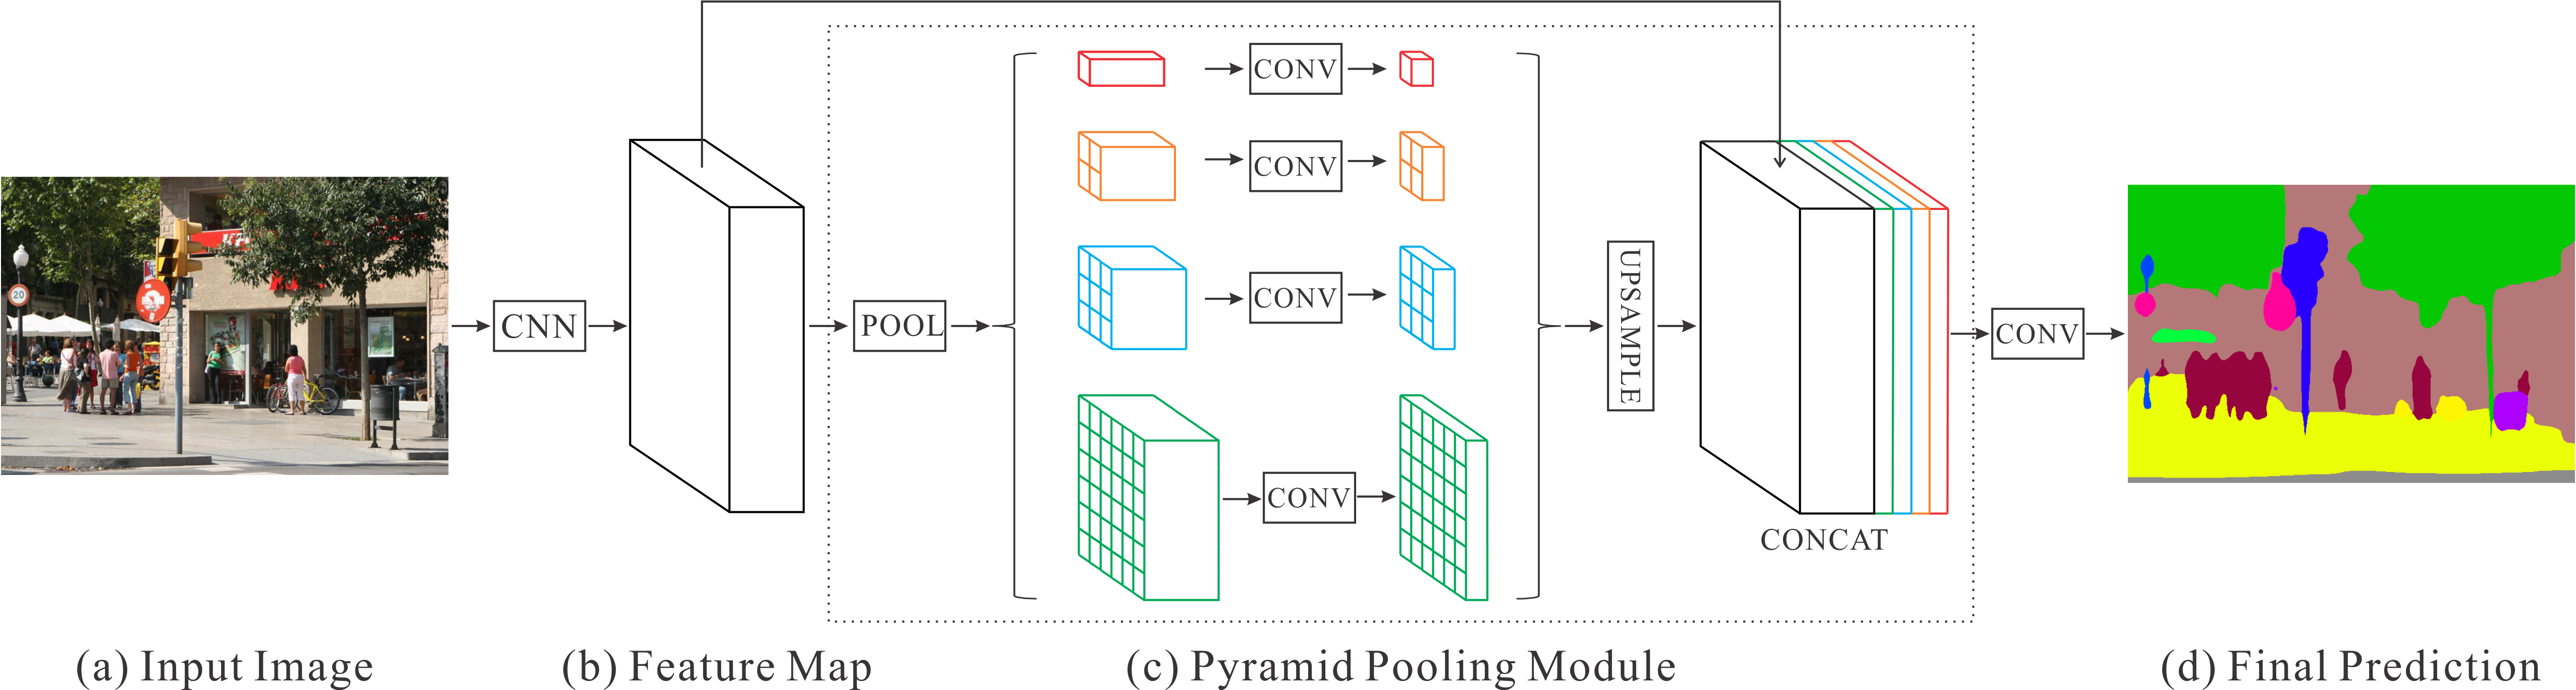
\includegraphics{wiki/pspnet.png}
\caption{pspnet}
\end{figure}

\begin{enumerate}
\def\labelenumi{\arabic{enumi}.}
\setcounter{enumi}{1}
\tightlist
\item
  \emph{Object Detection} is similar to the semantic segmentation but
  the difference is that only indicating a bounding box around the
  detected object would be enough (not pixel wise), but still objects in
  a image need to be detected. Note that if there are multiple instance
  of same object, still the bounding boxes and their labels must be
  distinct. So in simple words, classification and localization is done
  by object detection.
\end{enumerate}

\begin{figure}
\centering
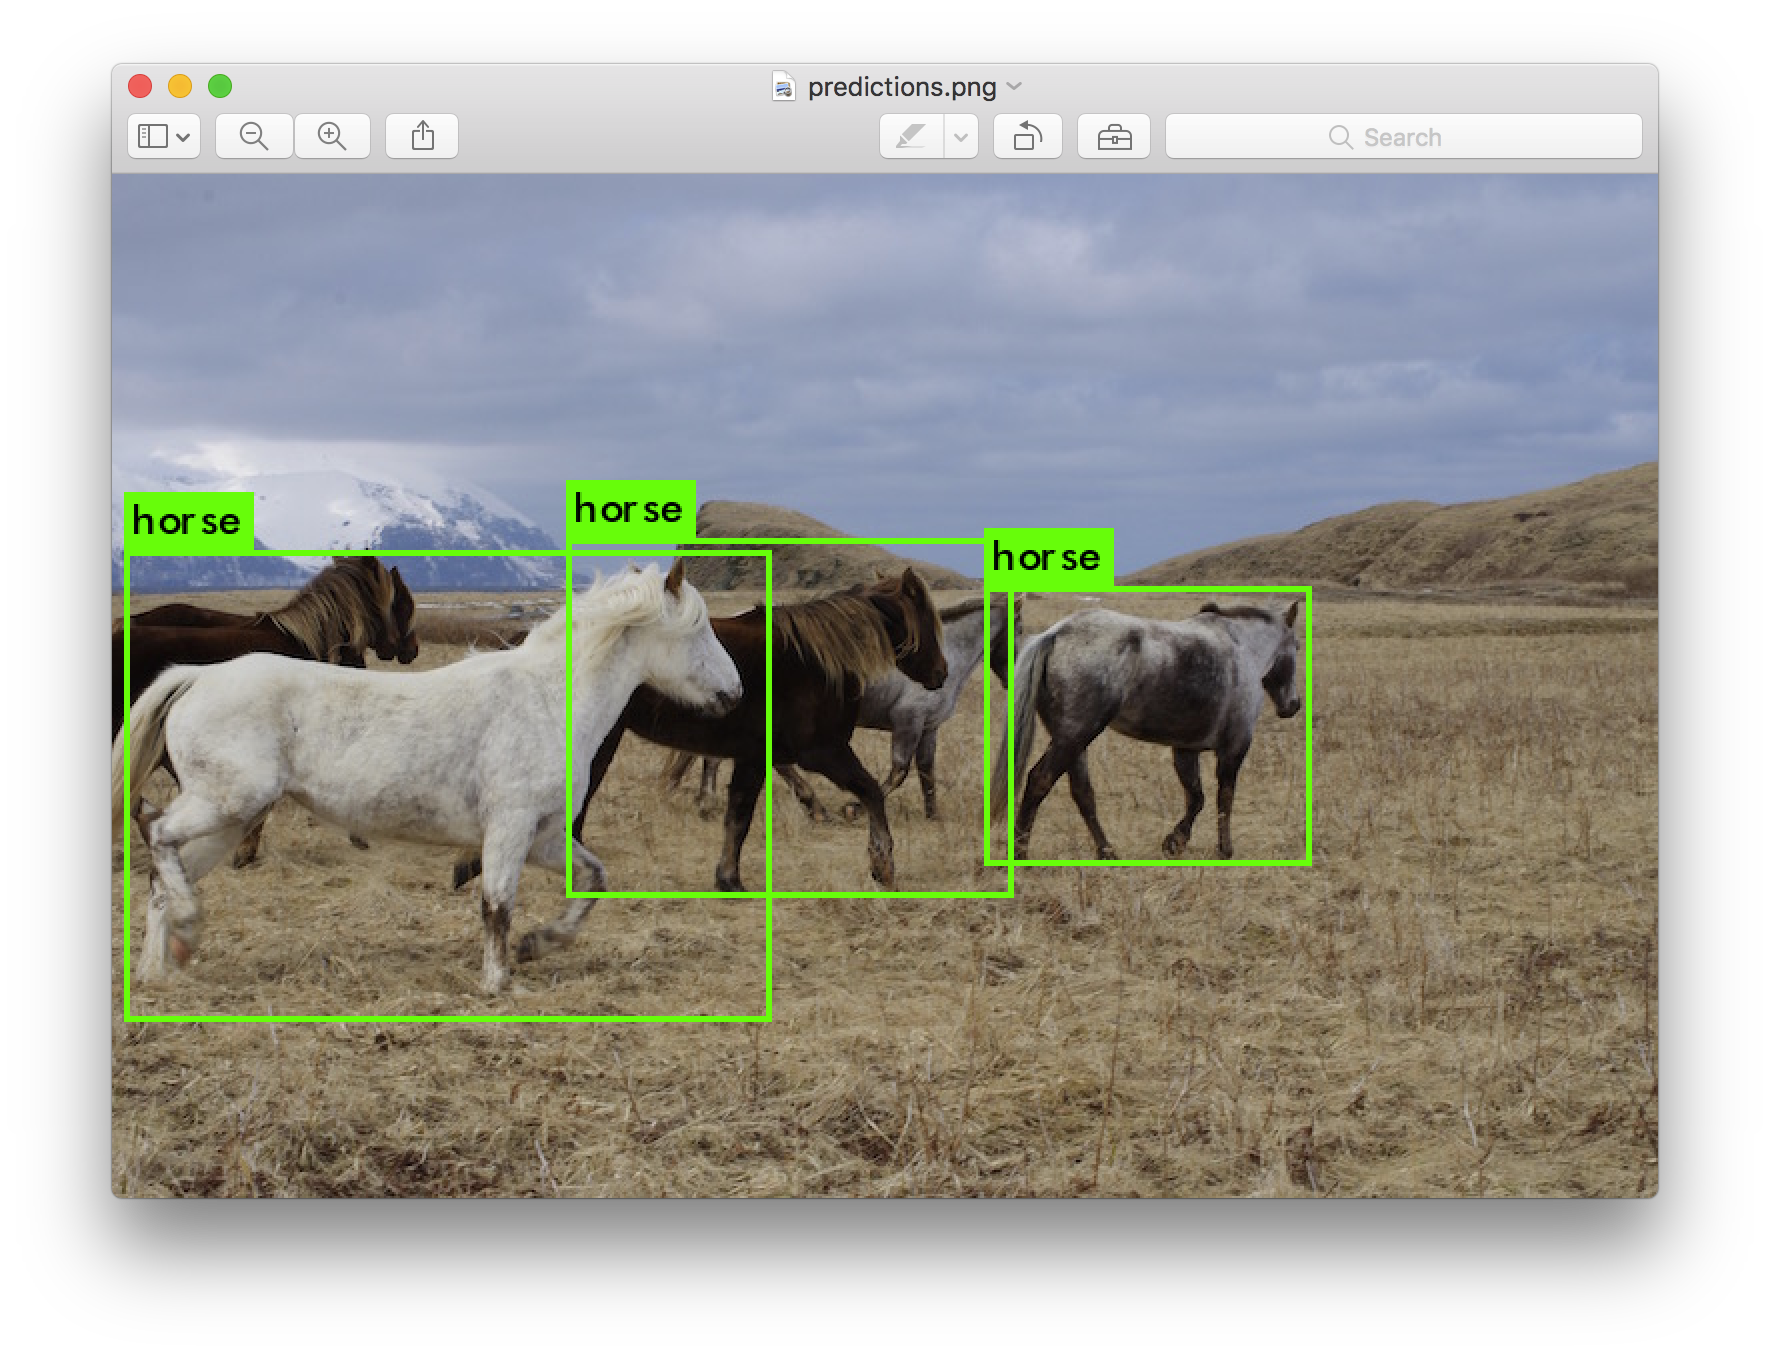
\includegraphics{wiki/objectdetection.png}
\caption{object detection}
\end{figure}

\begin{enumerate}
\def\labelenumi{\arabic{enumi}.}
\setcounter{enumi}{2}
\tightlist
\item
  \emph{Instance Segmentation} is similar to semantic segmenatation in
  term of pixel-wise classification but the major difference is that in
  semantic segmenation model is not aware of object or multiple instance
  of a same class, but in instance segmenatation, similar to object
  detection, all instance of same object need to be classified BUT
  pixel-wise.
\end{enumerate}

\begin{figure}
\centering
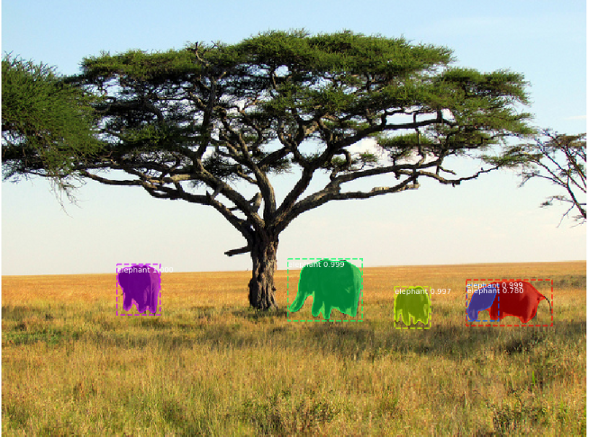
\includegraphics{wiki/instancesegmentation.png}
\caption{instance segmentation}
\end{figure}

    \hypertarget{compare-rcnn-fast-rcnn-and-faster-rcnn}{%
\subsection{\texorpdfstring{2 Compare \emph{RCNN}, \emph{Fast RCNN} and
\emph{Faster
RCNN}}{2 Compare RCNN, Fast RCNN and Faster RCNN}}\label{compare-rcnn-fast-rcnn-and-faster-rcnn}}

\begin{enumerate}
\def\labelenumi{\arabic{enumi}.}
\tightlist
\item
  RCNN
\item
  Fast RCNN
\item
  Faster RCNN
\end{enumerate}

    \hypertarget{a-rcnn}{%
\subsubsection{2.A RCNN}\label{a-rcnn}}

RCNN consists of two major components, a CNN and a Region extractor.

Firstly, it uses selective search to identify a rational number of
bounding boxes as the regions of interests (RoI). Seconly, It uses these
extracted regions as input to a pretrained CNN network for
classification separately.

\begin{figure}
\centering
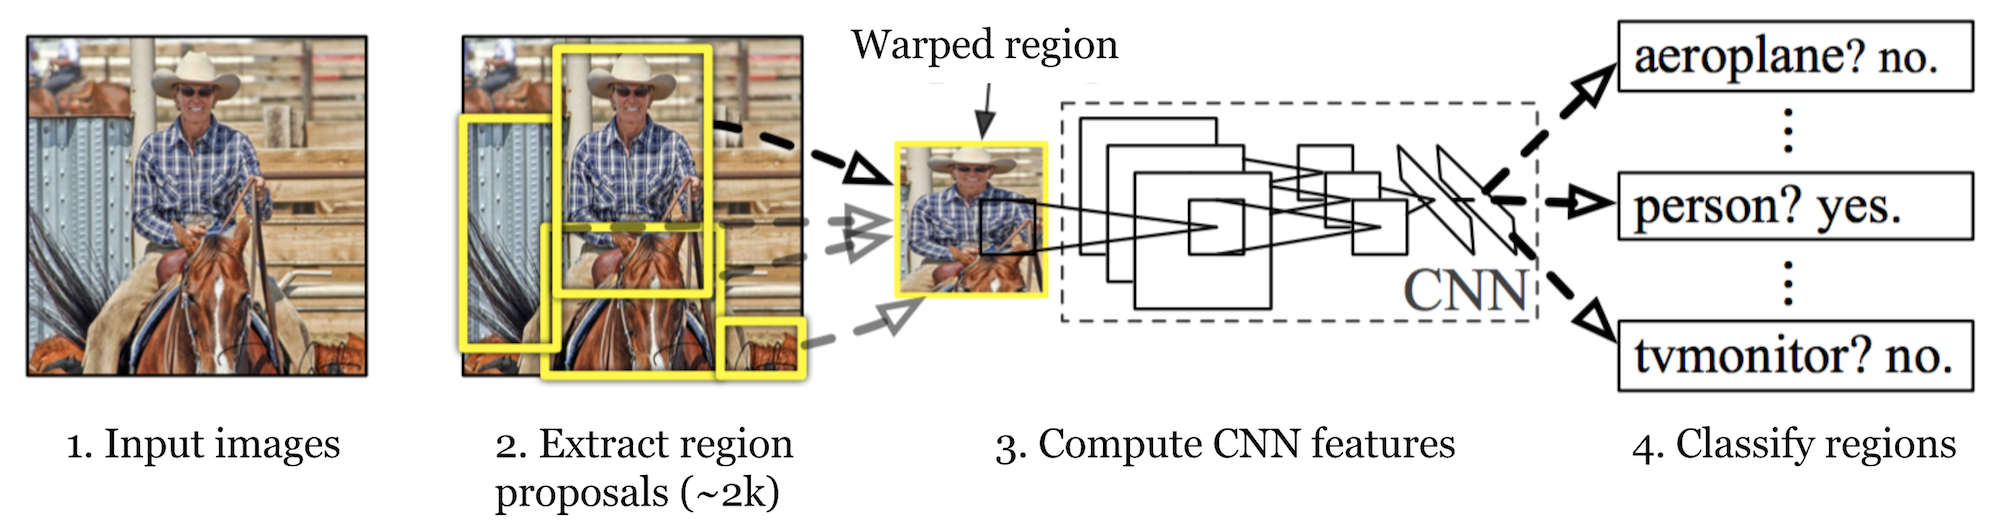
\includegraphics{wiki/rcnn1.png}
\caption{rcnn arch}
\end{figure}

Here are the main steps of RCNN:

\begin{enumerate}
\def\labelenumi{\arabic{enumi}.}
\tightlist
\item
  The CNN model must have been pretrained for a image classification
  tast such as VGG on ImageNet dataset
\item
  It uses RoI that is hardcoded and do not need to be optimized.
\item
  All extracted RoIs will be resized as the size of pretrained CNN
\item
  Fine tune the CNN model w.r.t. classes. But a point need to be
  mentioned is that as most of the proposed RoIs are negative samples,
  we need to oversample positive RoIs while fine tuning CNN model
\item
  Now we use CNN model to extract useful features from RoIs which in
  case of VGG it would be 4096 features
\item
  A binary SVM classfier (each class a distinct binary SVM) uses
  extracted features from CNN to classify the image
\item
  To find optimal localization, a regression model is used to to correct
  predicted boxes
\end{enumerate}

\begin{figure}
\centering
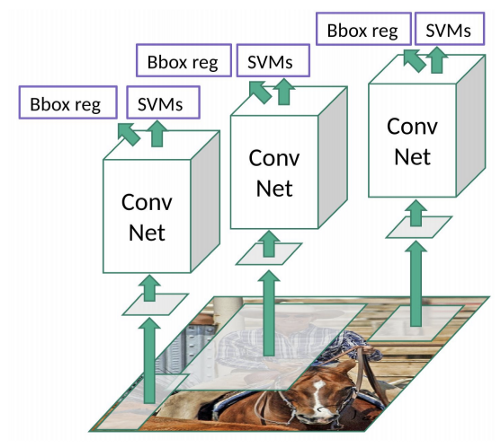
\includegraphics{wiki/rcnn2.png}
\caption{rcnn top down}
\end{figure}

The approach which Bounding Box Regressor takes: The BBregressor uses
predicted bounding box and ground truth to map in scale-variant manner.
Also it updates the height and width by learning log-scale
transformation. They used SSE loss plus L2 regularization to optimize
this regressor.

\begin{figure}
\centering
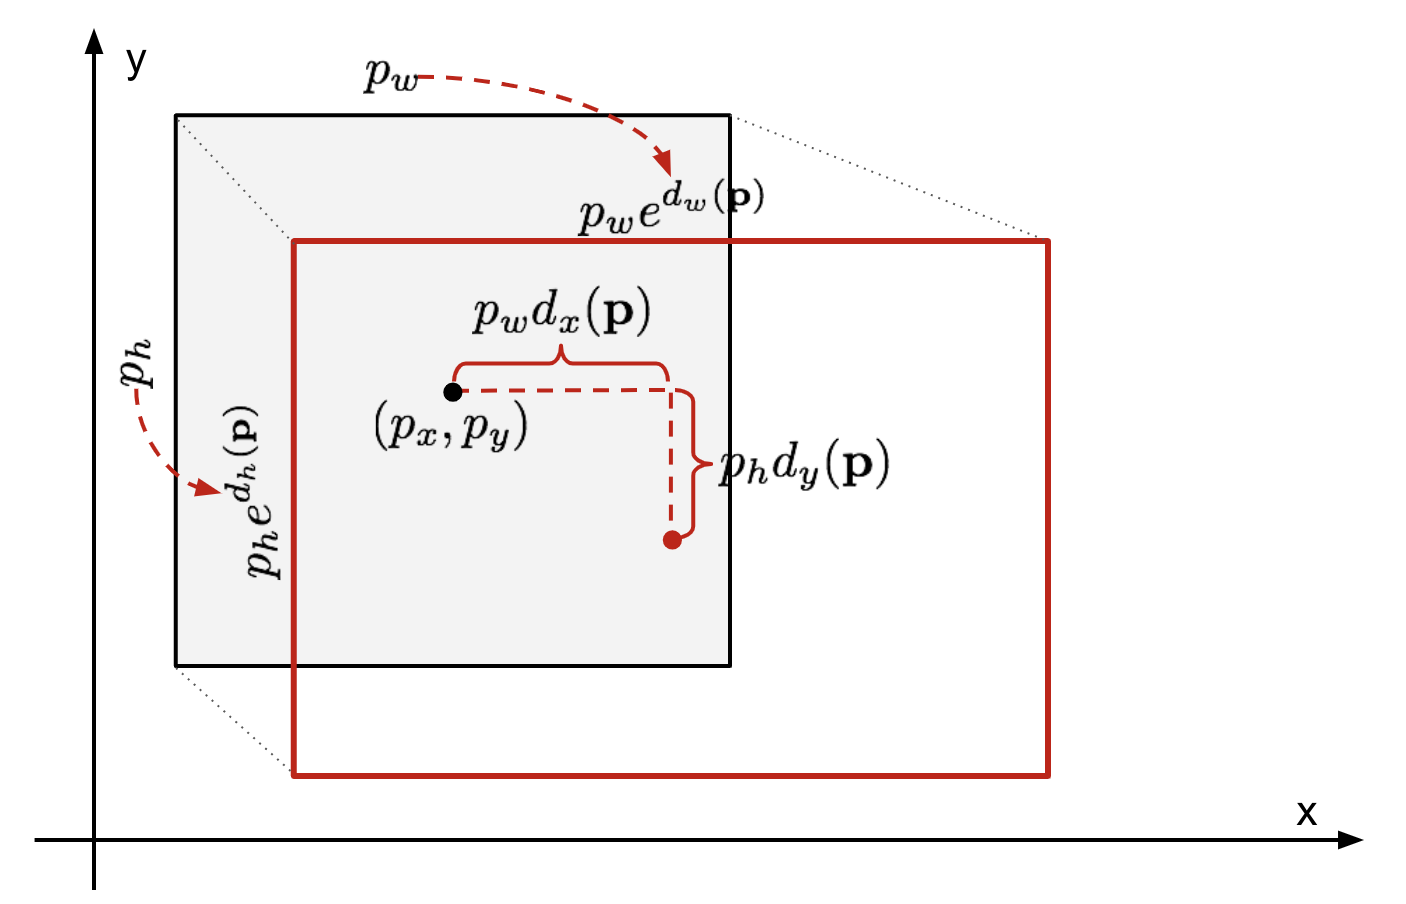
\includegraphics{wiki/rcnn3.png}
\caption{rcnn bb regressor}
\end{figure}

One important indication of RCNN is that they used Non-max suppression
to confluence overlapping bounding boxes into a single one which
represents more score than the others.

\begin{figure}
\centering
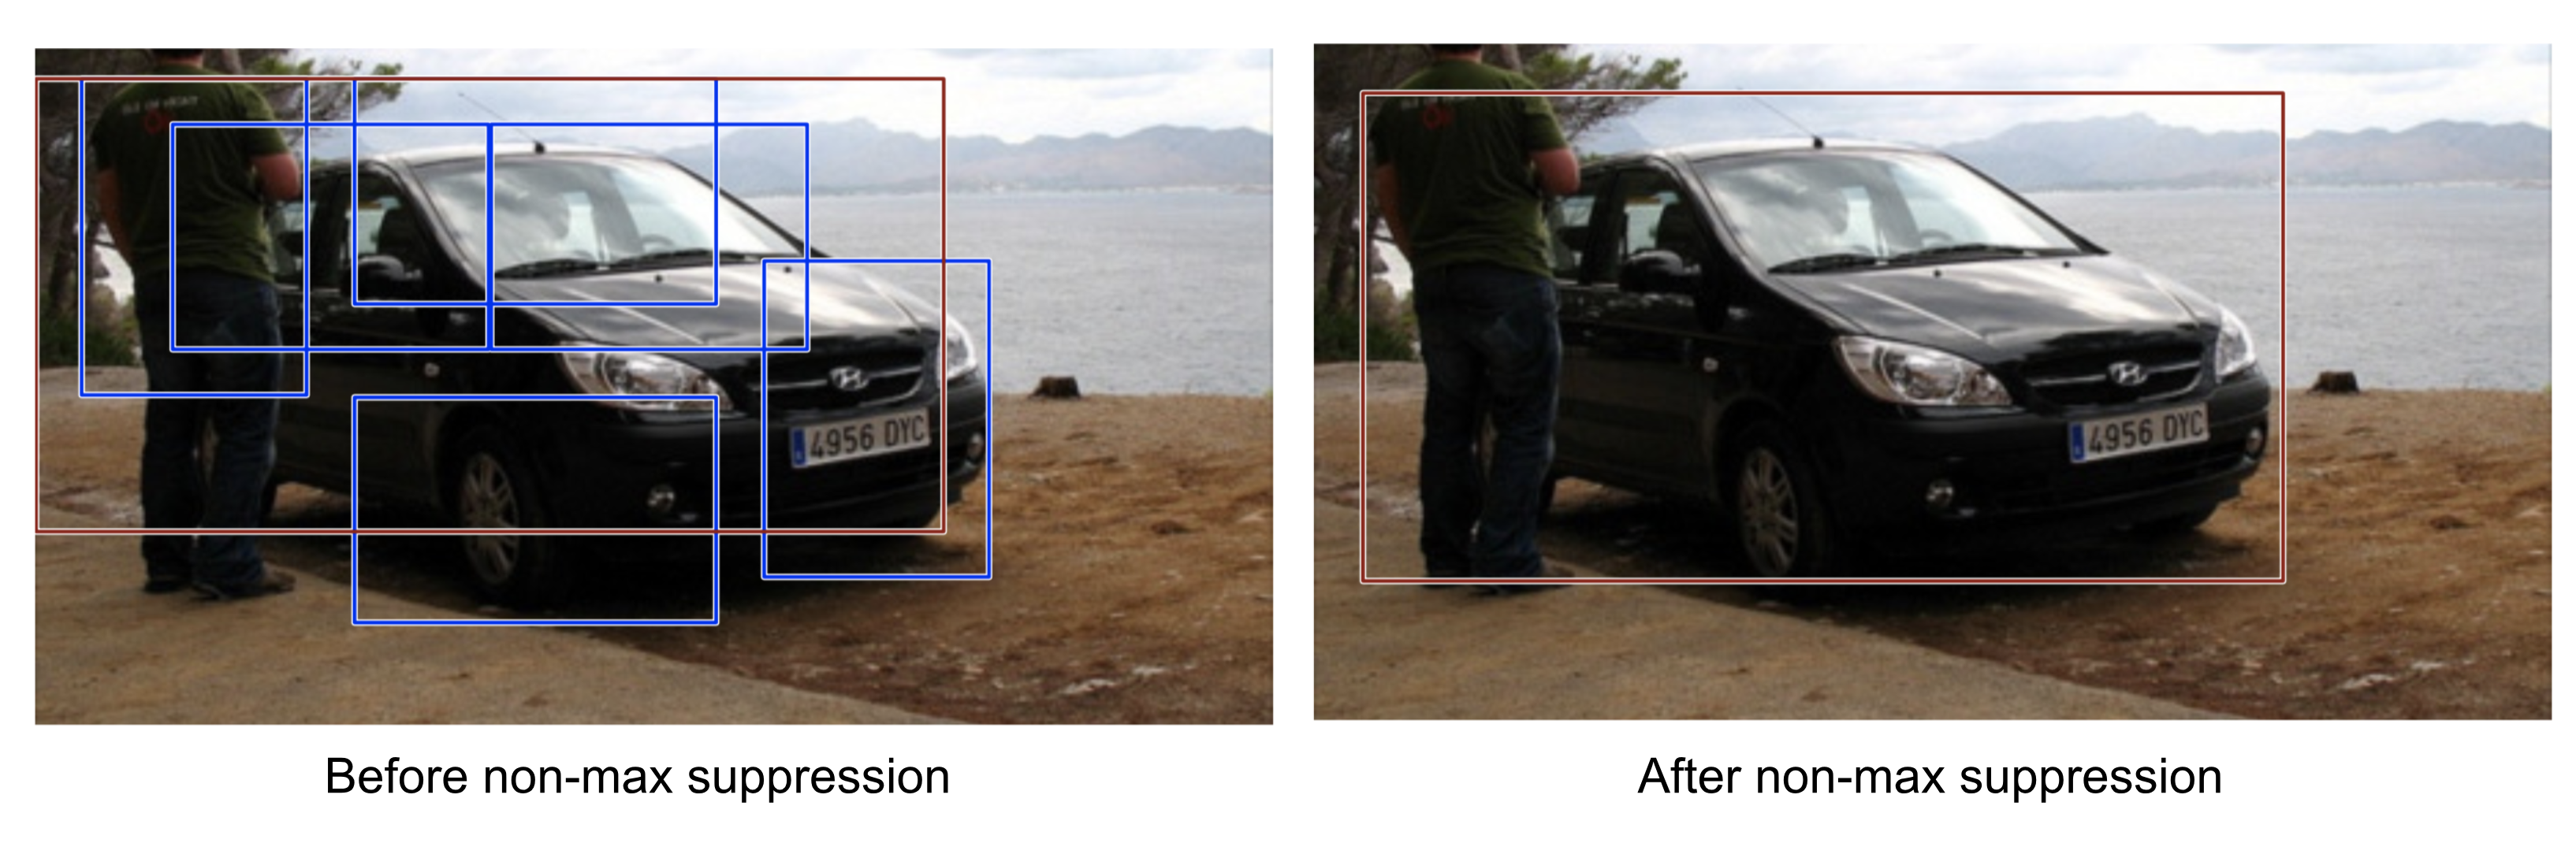
\includegraphics{wiki/nms.png}
\caption{nms}
\end{figure}

But this model has a lot of problems: 1. selective search has been used
to obtain RoIs which means it is not learnable and slow 2. For each
extracted RoI, CNN need to be called which makes the algorithm super
slow (about 47 sec per image) 3. All model are separate, regressor, CNN
and SVM!

    \hypertarget{b-fast-rcnn}{%
\subsubsection{2.B Fast RCNN}\label{b-fast-rcnn}}

What was the main problem of RCNN? Speed!

In fast RCNN, three distinct models joint each other to share results.
This model instead of using CNN independently for each extracted region,
it combines it with extraction part and only uses CNN once per image and
RoI is based on the feature of CNN. In other words, first we take CNN,
then RoI of feature vector generated from CNN and resize them to have
same size for all and finally a stacked neural nets are the structure.

\begin{figure}
\centering
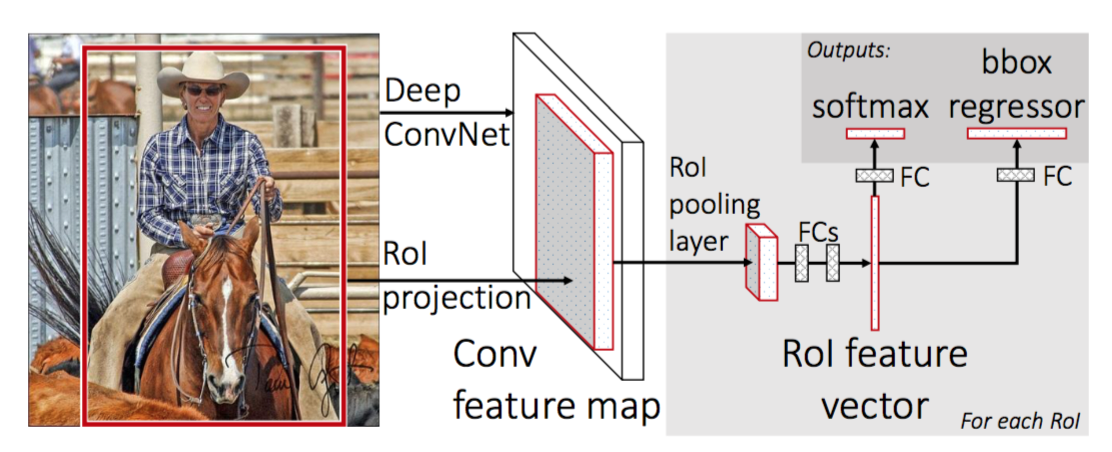
\includegraphics{wiki/fast1.png}
\caption{fast rcnn}
\end{figure}

This model to obtain the aforementioned approach, proposed a type of max
pooling called \emph{RoI Pooling}. This kind of pooling, decreases the
size of a feature image with region of interest to a smaller feature
image. It first make a grid with size of say hxw, then take max pooling
in each grid.

\begin{figure}
\centering
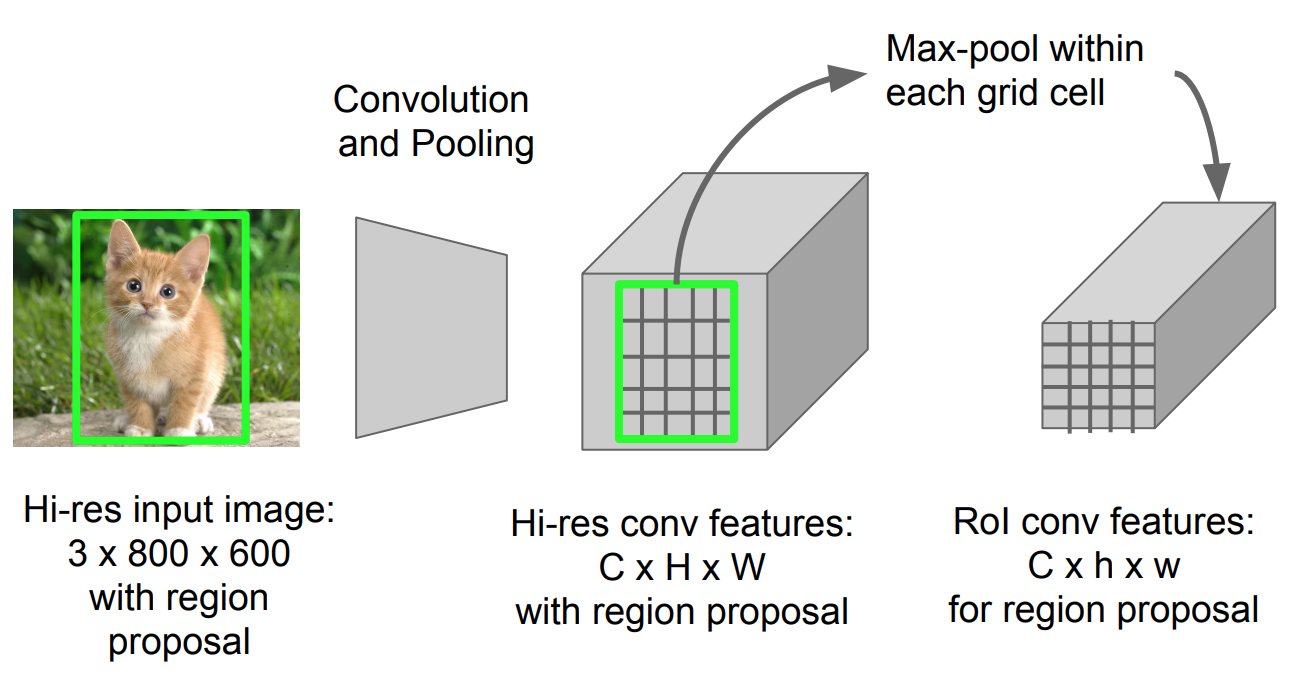
\includegraphics{wiki/fast2.png}
\caption{roi pooling}
\end{figure}

Most of the steps are same with RCNN so here are the main ones: 1. The
last pooling layer of CNN has been changed from max pooling to RoI
pooling. RoI pooling outputs fixed length feature vectors that can be
used for prediction perposes. 2. Last fully connected layer also needs
to be changed to support non-interest regions (background- non of our
classes) 3. This model also outputs two factors, first, score of
classifcation for each RoI, second, the bounding box value for
regressor. 4. Smooth L1 loss has been used for computing error of
bounding boxes. The overall loss function is sum of Smooth L1 and
softmax for classfication part.

The model has got much more speed since computation of models have been
shared and only once the CNN has been used instead of using it for each
RoI in each image. (N image=N*2000 CNN calls reduced to 1 CNN call!)

\begin{figure}
\centering
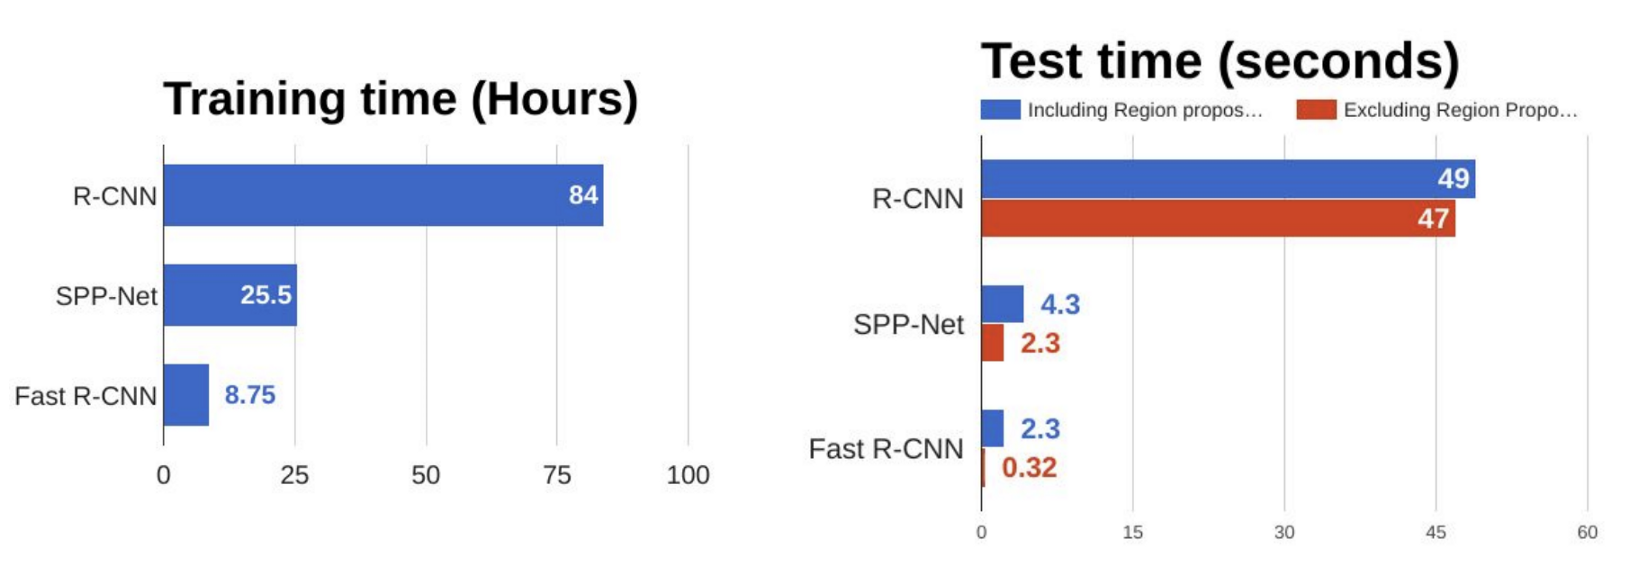
\includegraphics{wiki/fast3.png}
\caption{time compare rcnn fast rcnn}
\end{figure}

A big bottleneck can be seen in above image is that when using selective
search part to obtain RoIs, it almost take 2 seconds which is dominating
all other part of the network in fast RCNN. So you can guess what is
going to be in Faster RCNN!

\begin{figure}
\centering
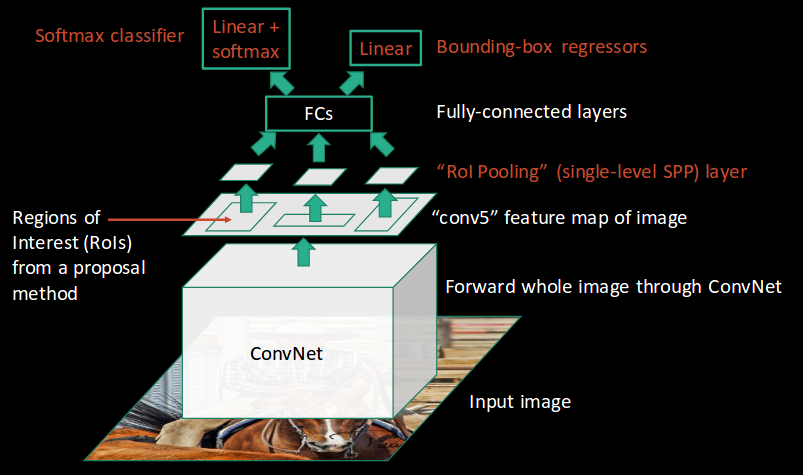
\includegraphics{wiki/fast4.png}
\caption{fast rcnn arch top down}
\end{figure}

    \hypertarget{c-faster-rcnn}{%
\subsubsection{2.C Faster RCNN}\label{c-faster-rcnn}}

The last line in Fast RCNN section told us that almost all delay in our
network is because of hardcoded part, the selective search for
extracting RoIs. So in simple words, Faster RCNN removed that part and
created a separate CNN model to extract RoIs from the given feature
vector and that is why we have an end-to-end network which is enormously
faster than hardcoded algorithms.

\begin{figure}
\centering
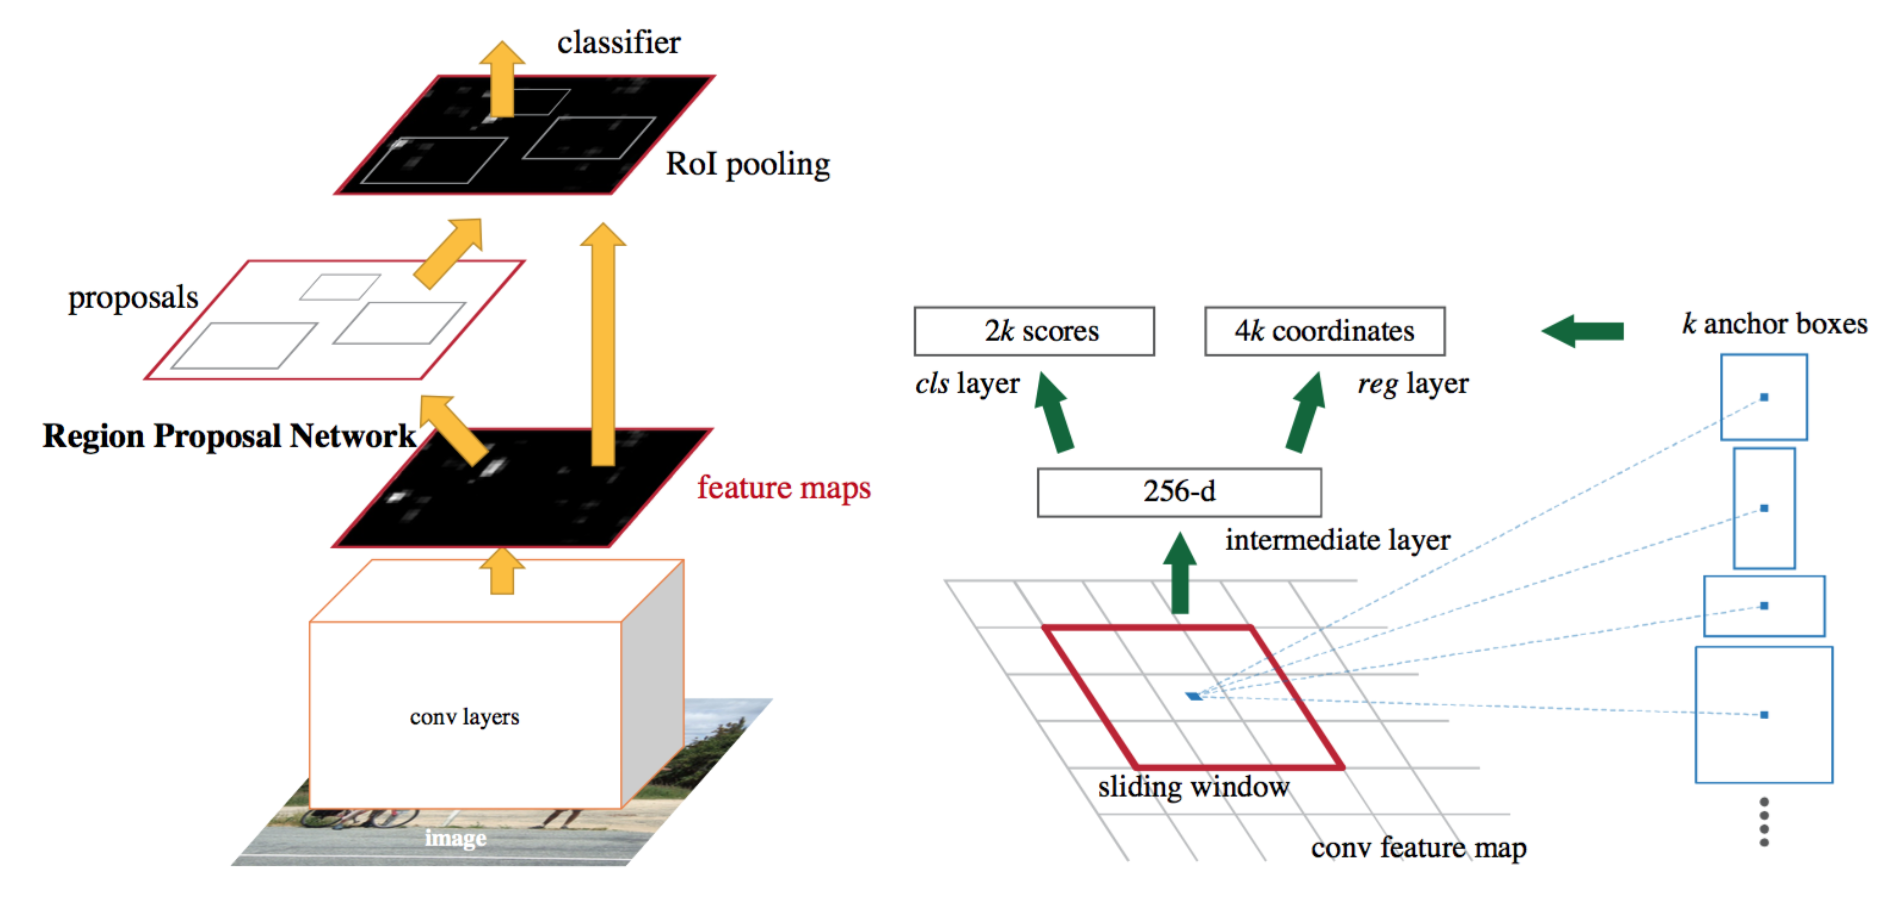
\includegraphics{wiki/faster1.png}
\caption{faster RCNN}
\end{figure}

How the model works: 1. Like always we need a pretrained CNN model 2.
Fine tune Region Proposal Network (the true heir of selective search!)
where has been initialized using the CNN pretrained model. RPN, slides
over the feature image obtained from pretrained CNN model, at each step
of sliding window of RPN, multiple region of various scale and ratios
are predicted simultaneously and the anchor is combination of these
predicted values. For instance, 3 scale, 3 ratios give us 9 anchor
boxes.

\begin{figure}
\centering
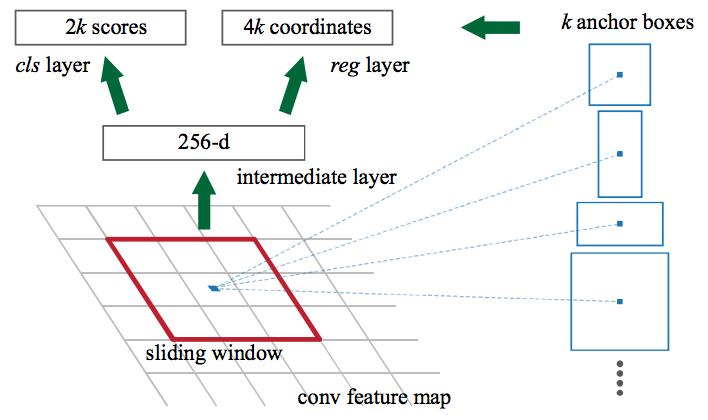
\includegraphics{wiki/faster4.png}
\caption{RPN}
\end{figure}

\begin{enumerate}
\def\labelenumi{\arabic{enumi}.}
\setcounter{enumi}{2}
\tightlist
\item
  Reshape extracted regions by RoI pooling layer
\item
  Train FAST RCNN using currently proposed RoIs by RPN.
\item
  Use FAST RCNN network which has been trained in previous step for
  initializing RPN, and only fine tune layers specifictly for RPN as RPN
  and predictor have common layers.
\item
  Freeze RPN and fine tune layers uniquely of the Fast RCNN (exclude
  common layers).
\end{enumerate}

\begin{figure}
\centering
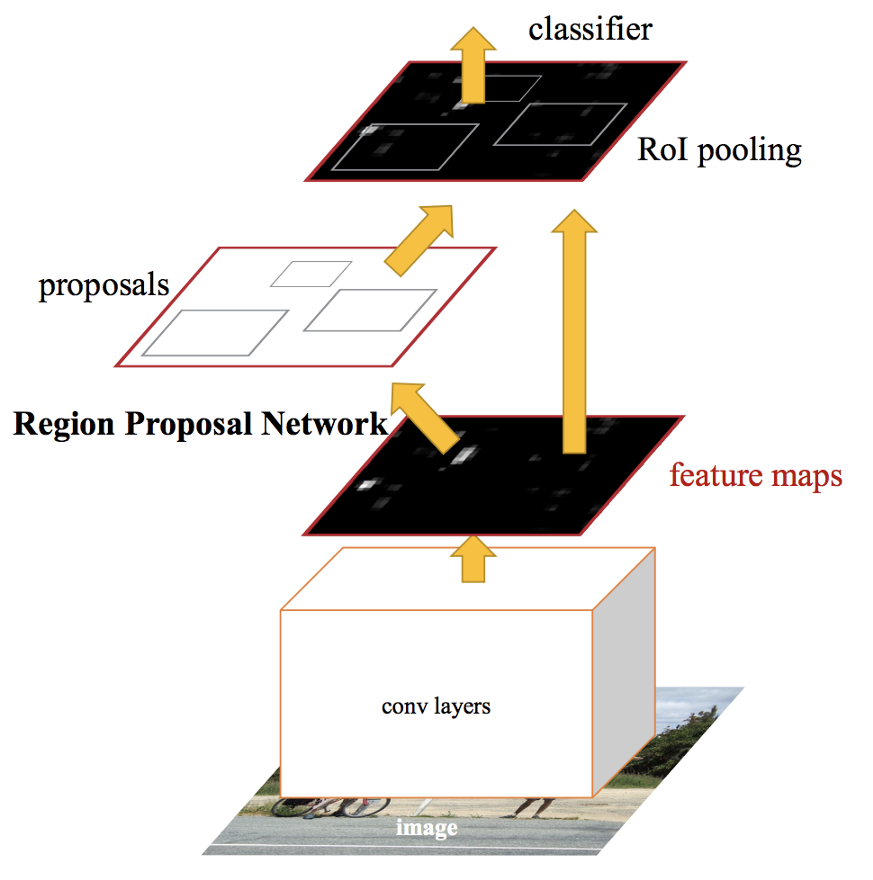
\includegraphics{wiki/faster2.png}
\caption{faster RCNN top down arch}
\end{figure}

In this model aslo a value of score that current predicted anchor is
indicating an object plus attribute of the bounding box is the inputs of
loss function where loss function are same with Fast RCNN.

This approach enabled model to skip the bottleneck of using selective
search. Here is the time and performance imporovemenets:

\begin{figure}
\centering
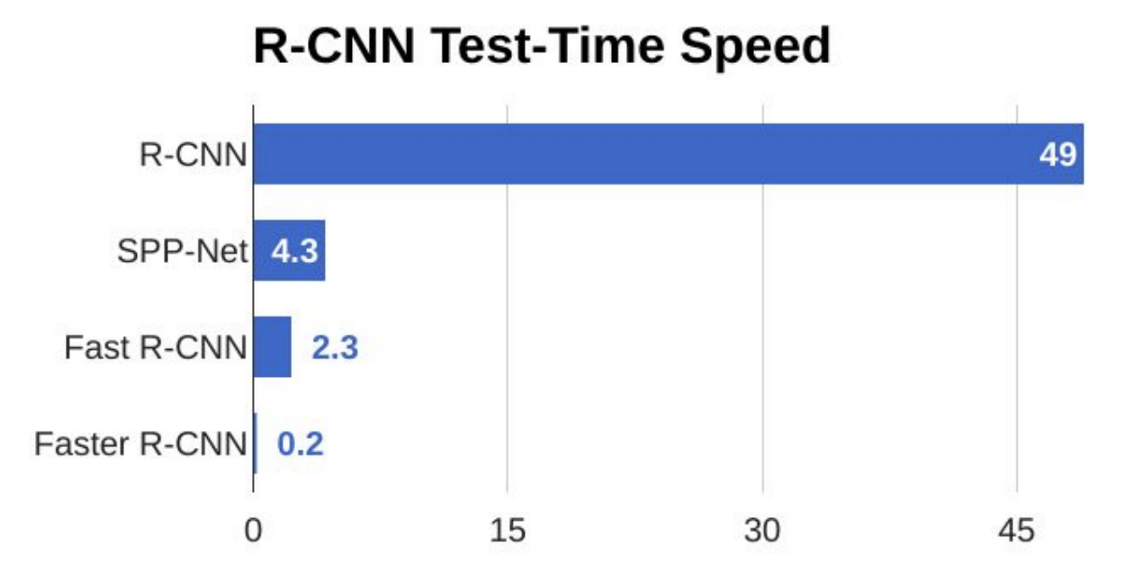
\includegraphics{wiki/faster3.png}
\caption{faster RCNN time consumption}
\end{figure}

    \hypertarget{car-plate-reader-via-matching-template}{%
\subsection{3 Car Plate Reader via Matching
Template}\label{car-plate-reader-via-matching-template}}

\begin{enumerate}
\def\labelenumi{\arabic{enumi}.}
\tightlist
\item
  Libraries
\item
  First Approach
\item
  Second Approach (didn't finished!)
\end{enumerate}

    \hypertarget{a-libraries}{%
\subsubsection{3.A Libraries}\label{a-libraries}}

    \begin{Verbatim}[commandchars=\\\{\}]
{\color{incolor}In [{\color{incolor}172}]:} \PY{k+kn}{import} \PY{n+nn}{cv2}
          \PY{k+kn}{import} \PY{n+nn}{matplotlib}\PY{n+nn}{.}\PY{n+nn}{pyplot} \PY{k}{as} \PY{n+nn}{plt}
          \PY{k+kn}{import} \PY{n+nn}{numpy} \PY{k}{as} \PY{n+nn}{np}
          \PY{k+kn}{from} \PY{n+nn}{skimage}\PY{n+nn}{.}\PY{n+nn}{feature} \PY{k}{import} \PY{n}{match\PYZus{}template}
          \PY{k+kn}{from} \PY{n+nn}{sklearn}\PY{n+nn}{.}\PY{n+nn}{cluster} \PY{k}{import} \PY{n}{DBSCAN}
          
          \PY{o}{\PYZpc{}}\PY{k}{matplotlib} inline
\end{Verbatim}


    \hypertarget{b-first-approach}{%
\subsubsection{3.B First Approach}\label{b-first-approach}}

Reading each character using a threshold distinctly from other
characters, then finding their locations using clustering techniques
such as DBSCAN instead of non-max suppression using IoU. 1. Setting
Hyper parameters 2. Preprocessing image 3. Iterating over and
preprocessing templates

    \hypertarget{b.a-setting-hyper-parameters}{%
\paragraph{3.B.a Setting hyper
parameters}\label{b.a-setting-hyper-parameters}}

    \begin{Verbatim}[commandchars=\\\{\}]
{\color{incolor}In [{\color{incolor} }]:} \PY{n}{NUMBER\PYZus{}COUNTS} \PY{o}{=} \PY{l+m+mi}{9}
        
        \PY{n}{rotation\PYZus{}angles} \PY{o}{=} \PY{p}{[}\PY{o}{\PYZhy{}}\PY{l+m+mi}{20}\PY{p}{,} \PY{o}{\PYZhy{}}\PY{l+m+mi}{15}\PY{p}{,} \PY{o}{\PYZhy{}}\PY{l+m+mi}{10}\PY{p}{,} \PY{o}{\PYZhy{}}\PY{l+m+mi}{5}\PY{p}{,} \PY{l+m+mi}{0}\PY{p}{,} \PY{l+m+mi}{5}\PY{p}{,} \PY{l+m+mi}{10}\PY{p}{,} \PY{l+m+mi}{15}\PY{p}{,} \PY{l+m+mi}{20}\PY{p}{]}
        \PY{n}{scale\PYZus{}percents} \PY{o}{=} \PY{p}{[}\PY{l+m+mi}{10}\PY{p}{,} \PY{l+m+mi}{20}\PY{p}{,} \PY{l+m+mi}{30}\PY{p}{,} \PY{l+m+mi}{40}\PY{p}{,} \PY{l+m+mi}{50}\PY{p}{,} \PY{l+m+mi}{70}\PY{p}{,} \PY{l+m+mi}{80}\PY{p}{,} \PY{l+m+mi}{90}\PY{p}{,} \PY{l+m+mi}{100}\PY{p}{,} \PY{l+m+mi}{110}\PY{p}{]}
        \PY{n}{threshold} \PY{o}{=} \PY{l+m+mf}{0.7}
\end{Verbatim}


    \hypertarget{b.b-preprocessing-image}{%
\paragraph{3.B.b Preprocessing Image}\label{b.b-preprocessing-image}}

    \begin{Verbatim}[commandchars=\\\{\}]
{\color{incolor}In [{\color{incolor} }]:} \PY{n}{img} \PY{o}{=} \PY{n}{cv2}\PY{o}{.}\PY{n}{imread}\PY{p}{(}\PY{l+s+s1}{\PYZsq{}}\PY{l+s+s1}{plates/Plate5.jpg}\PY{l+s+s1}{\PYZsq{}}\PY{p}{)}
        \PY{n}{img} \PY{o}{=} \PY{n}{cv2}\PY{o}{.}\PY{n}{cvtColor}\PY{p}{(}\PY{n}{img}\PY{p}{,} \PY{n}{cv2}\PY{o}{.}\PY{n}{COLOR\PYZus{}BGR2GRAY}\PY{p}{)}
        \PY{p}{(}\PY{n}{\PYZus{}}\PY{p}{,} \PY{n}{img}\PY{p}{)} \PY{o}{=} \PY{n}{cv2}\PY{o}{.}\PY{n}{threshold}\PY{p}{(}\PY{n}{img}\PY{p}{,} \PY{l+m+mi}{128}\PY{p}{,} \PY{l+m+mi}{255}\PY{p}{,} \PY{n}{cv2}\PY{o}{.}\PY{n}{THRESH\PYZus{}BINARY} \PY{o}{|} \PY{n}{cv2}\PY{o}{.}\PY{n}{THRESH\PYZus{}OTSU}\PY{p}{)}
\end{Verbatim}


    \hypertarget{b.c-iterating-over-and-preprocessing-templates}{%
\paragraph{3.B.c Iterating over and preprocessing
templates}\label{b.c-iterating-over-and-preprocessing-templates}}

    \begin{Verbatim}[commandchars=\\\{\}]
{\color{incolor}In [{\color{incolor}292}]:} \PY{n}{num\PYZus{}pos} \PY{o}{=} \PY{n}{np}\PY{o}{.}\PY{n}{ones}\PY{p}{(}\PY{n}{NUMBER\PYZus{}COUNTS}\PY{p}{)} \PY{o}{*} \PY{o}{\PYZhy{}}\PY{l+m+mi}{1}
          
          \PY{k}{for} \PY{n}{template\PYZus{}number} \PY{o+ow}{in} \PY{n+nb}{range}\PY{p}{(}\PY{l+m+mi}{10}\PY{p}{)}\PY{p}{:}
              \PY{n}{template} \PY{o}{=} \PY{n}{cv2}\PY{o}{.}\PY{n}{imread}\PY{p}{(}\PY{l+s+s1}{\PYZsq{}}\PY{l+s+s1}{Templates/}\PY{l+s+s1}{\PYZsq{}}\PY{o}{+}\PY{n+nb}{str}\PY{p}{(}\PY{n}{template\PYZus{}number}\PY{p}{)}\PY{o}{+}\PY{l+s+s1}{\PYZsq{}}\PY{l+s+s1}{.jpg}\PY{l+s+s1}{\PYZsq{}}\PY{p}{)}
              \PY{n}{template} \PY{o}{=} \PY{n}{cv2}\PY{o}{.}\PY{n}{cvtColor}\PY{p}{(}\PY{n}{template}\PY{p}{,} \PY{n}{cv2}\PY{o}{.}\PY{n}{COLOR\PYZus{}BGR2GRAY}\PY{p}{)}
              \PY{p}{(}\PY{n}{\PYZus{}}\PY{p}{,} \PY{n}{template}\PY{p}{)} \PY{o}{=} \PY{n}{cv2}\PY{o}{.}\PY{n}{threshold}\PY{p}{(}\PY{n}{template}\PY{p}{,} \PY{l+m+mi}{128}\PY{p}{,} \PY{l+m+mi}{255}\PY{p}{,} \PY{n}{cv2}\PY{o}{.}\PY{n}{THRESH\PYZus{}BINARY} \PY{o}{|} \PY{n}{cv2}\PY{o}{.}\PY{n}{THRESH\PYZus{}OTSU}\PY{p}{)}
          
              \PY{k}{for} \PY{n}{scale} \PY{o+ow}{in} \PY{n}{scale\PYZus{}percents}\PY{p}{:}
                  \PY{k}{for} \PY{n}{angle} \PY{o+ow}{in} \PY{n}{rotation\PYZus{}angles}\PY{p}{:}
                      \PY{c+c1}{\PYZsh{} resize}
                      \PY{n}{width} \PY{o}{=} \PY{n+nb}{int}\PY{p}{(}\PY{n}{template}\PY{o}{.}\PY{n}{shape}\PY{p}{[}\PY{l+m+mi}{1}\PY{p}{]} \PY{o}{*} \PY{n}{scale} \PY{o}{/} \PY{l+m+mi}{100}\PY{p}{)}
                      \PY{n}{height} \PY{o}{=} \PY{n+nb}{int}\PY{p}{(}\PY{n}{template}\PY{o}{.}\PY{n}{shape}\PY{p}{[}\PY{l+m+mi}{0}\PY{p}{]} \PY{o}{*} \PY{n}{scale} \PY{o}{/} \PY{l+m+mi}{100}\PY{p}{)}
                      \PY{n}{dim} \PY{o}{=} \PY{p}{(}\PY{n}{width}\PY{p}{,} \PY{n}{height}\PY{p}{)}
                      \PY{n}{temp} \PY{o}{=} \PY{n}{cv2}\PY{o}{.}\PY{n}{resize}\PY{p}{(}\PY{n}{template}\PY{p}{,} \PY{n}{dim}\PY{p}{,} \PY{n}{interpolation} \PY{o}{=} \PY{n}{cv2}\PY{o}{.}\PY{n}{INTER\PYZus{}AREA}\PY{p}{)}
                      \PY{k}{if} \PY{n}{temp}\PY{o}{.}\PY{n}{shape}\PY{p}{[}\PY{l+m+mi}{0}\PY{p}{]} \PY{o}{\PYZgt{}} \PY{n}{img}\PY{o}{.}\PY{n}{shape}\PY{p}{[}\PY{l+m+mi}{0}\PY{p}{]} \PY{o+ow}{or} \PY{n}{temp}\PY{o}{.}\PY{n}{shape}\PY{p}{[}\PY{l+m+mi}{1}\PY{p}{]} \PY{o}{\PYZgt{}} \PY{n}{img}\PY{o}{.}\PY{n}{shape}\PY{p}{[}\PY{l+m+mi}{1}\PY{p}{]}\PY{p}{:}
                          \PY{k}{continue}
                      \PY{c+c1}{\PYZsh{} rotate}
                      \PY{n}{temp\PYZus{}center} \PY{o}{=} \PY{n+nb}{tuple}\PY{p}{(}\PY{n}{np}\PY{o}{.}\PY{n}{array}\PY{p}{(}\PY{n}{temp}\PY{o}{.}\PY{n}{shape}\PY{p}{[}\PY{l+m+mi}{1}\PY{p}{:}\PY{p}{:}\PY{o}{\PYZhy{}}\PY{l+m+mi}{1}\PY{p}{]}\PY{p}{)} \PY{o}{/} \PY{l+m+mi}{2}\PY{p}{)}
                      \PY{n}{rot\PYZus{}mat} \PY{o}{=} \PY{n}{cv2}\PY{o}{.}\PY{n}{getRotationMatrix2D}\PY{p}{(}\PY{n}{temp\PYZus{}center}\PY{p}{,} \PY{n}{angle}\PY{p}{,} \PY{l+m+mf}{1.0}\PY{p}{)}
                      \PY{n}{result} \PY{o}{=} \PY{n}{cv2}\PY{o}{.}\PY{n}{warpAffine}\PY{p}{(}\PY{n}{temp}\PY{p}{,} \PY{n}{rot\PYZus{}mat}\PY{p}{,} \PY{n}{temp}\PY{o}{.}\PY{n}{shape}\PY{p}{[}\PY{l+m+mi}{1}\PY{p}{:}\PY{p}{:}\PY{o}{\PYZhy{}}\PY{l+m+mi}{1}\PY{p}{]}\PY{p}{,} \PY{n}{flags}\PY{o}{=}\PY{n}{cv2}\PY{o}{.}\PY{n}{INTER\PYZus{}LINEAR}\PY{p}{,} \PY{n}{borderValue}\PY{o}{=}\PY{p}{(}\PY{l+m+mi}{255}\PY{p}{,}\PY{l+m+mi}{255}\PY{p}{,}\PY{l+m+mi}{255}\PY{p}{)}\PY{p}{)}
                      \PY{n}{w}\PY{p}{,} \PY{n}{h} \PY{o}{=} \PY{n}{temp}\PY{o}{.}\PY{n}{shape}\PY{p}{[}\PY{p}{:}\PY{p}{:}\PY{o}{\PYZhy{}}\PY{l+m+mi}{1}\PY{p}{]}
                      
                      \PY{c+c1}{\PYZsh{} template matching}
                      \PY{n}{res} \PY{o}{=} \PY{n}{cv2}\PY{o}{.}\PY{n}{matchTemplate}\PY{p}{(}\PY{n}{img}\PY{p}{,} \PY{n}{temp}\PY{p}{,} \PY{n}{cv2}\PY{o}{.}\PY{n}{TM\PYZus{}CCOEFF\PYZus{}NORMED}\PY{p}{)}
                      \PY{n}{loc} \PY{o}{=} \PY{n}{np}\PY{o}{.}\PY{n}{where}\PY{p}{(} \PY{n}{res} \PY{o}{\PYZgt{}}\PY{o}{=} \PY{n}{threshold}\PY{p}{)}
                      \PY{k}{if} \PY{o+ow}{not} \PY{n}{loc}\PY{p}{[}\PY{l+m+mi}{1}\PY{p}{]}\PY{o}{.}\PY{n}{shape}\PY{p}{[}\PY{l+m+mi}{0}\PY{p}{]} \PY{o}{==} \PY{l+m+mi}{0}\PY{p}{:}
                          \PY{n}{dbscan} \PY{o}{=} \PY{n}{DBSCAN}\PY{p}{(}\PY{n}{eps}\PY{o}{=}\PY{l+m+mi}{3}\PY{p}{)}
                          \PY{n}{dbscan}\PY{o}{.}\PY{n}{fit}\PY{p}{(}\PY{n}{loc}\PY{p}{[}\PY{l+m+mi}{1}\PY{p}{]}\PY{o}{.}\PY{n}{reshape}\PY{p}{(}\PY{o}{\PYZhy{}}\PY{l+m+mi}{1}\PY{p}{,} \PY{l+m+mi}{1}\PY{p}{)}\PY{p}{)}
                          \PY{k}{for} \PY{n}{cluster} \PY{o+ow}{in} \PY{n+nb}{range}\PY{p}{(}\PY{n}{dbscan}\PY{o}{.}\PY{n}{labels\PYZus{}}\PY{o}{.}\PY{n}{max}\PY{p}{(}\PY{p}{)}\PY{o}{+}\PY{l+m+mi}{1}\PY{p}{)}\PY{p}{:}
                              \PY{n}{idx} \PY{o}{=} \PY{n}{loc}\PY{p}{[}\PY{l+m+mi}{1}\PY{p}{]}\PY{p}{[}\PY{p}{(}\PY{n}{dbscan}\PY{o}{.}\PY{n}{labels\PYZus{}} \PY{o}{==} \PY{n}{cluster}\PY{p}{)}\PY{o}{.}\PY{n}{nonzero}\PY{p}{(}\PY{p}{)}\PY{p}{[}\PY{l+m+mi}{0}\PY{p}{]}\PY{p}{]}\PY{o}{.}\PY{n}{mean}\PY{p}{(}\PY{p}{)} \PY{o}{/}\PY{o}{/} \PY{p}{(}\PY{n}{img}\PY{o}{.}\PY{n}{shape}\PY{p}{[}\PY{l+m+mi}{1}\PY{p}{]} \PY{o}{/} \PY{n}{NUMBER\PYZus{}COUNTS}\PY{p}{)}
                              \PY{n}{num\PYZus{}pos}\PY{p}{[}\PY{n+nb}{int}\PY{p}{(}\PY{n}{idx}\PY{p}{)}\PY{p}{]} \PY{o}{=} \PY{n}{template\PYZus{}number}
                              \PY{c+c1}{\PYZsh{} here use \PYZsq{}res\PYZsq{} and \PYZsq{}idx\PYZsq{} to get maximum probability then apply template number with max res value}
                          \PY{k}{for} \PY{n}{pt} \PY{o+ow}{in} \PY{n+nb}{zip}\PY{p}{(}\PY{o}{*}\PY{n}{loc}\PY{p}{[}\PY{p}{:}\PY{p}{:}\PY{o}{\PYZhy{}}\PY{l+m+mi}{1}\PY{p}{]}\PY{p}{)}\PY{p}{:}
                              \PY{n}{cv2}\PY{o}{.}\PY{n}{rectangle}\PY{p}{(}\PY{n}{img}\PY{p}{,} \PY{n}{pt}\PY{p}{,} \PY{p}{(}\PY{n}{pt}\PY{p}{[}\PY{l+m+mi}{0}\PY{p}{]} \PY{o}{+} \PY{n}{w}\PY{p}{,} \PY{n}{pt}\PY{p}{[}\PY{l+m+mi}{1}\PY{p}{]} \PY{o}{+} \PY{n}{h}\PY{p}{)}\PY{p}{,} \PY{p}{(}\PY{l+m+mi}{0}\PY{p}{,}\PY{l+m+mi}{0}\PY{p}{,}\PY{l+m+mi}{255}\PY{p}{)}\PY{p}{,} \PY{l+m+mi}{1}\PY{p}{)}
                          \PY{n}{cv2}\PY{o}{.}\PY{n}{imwrite}\PY{p}{(}\PY{l+s+s1}{\PYZsq{}}\PY{l+s+s1}{res.png}\PY{l+s+s1}{\PYZsq{}}\PY{p}{,} \PY{n}{img}\PY{p}{)}
          \PY{k}{if} \PY{n}{num\PYZus{}pos}\PY{p}{[}\PY{l+m+mi}{0}\PY{p}{]} \PY{o}{!=} \PY{o}{\PYZhy{}}\PY{l+m+mi}{1}\PY{p}{:}
              \PY{n}{num\PYZus{}pos}\PY{p}{[}\PY{l+m+mi}{1}\PY{p}{]} \PY{o}{=} \PY{n}{num\PYZus{}pos}\PY{p}{[}\PY{l+m+mi}{0}\PY{p}{]}
              \PY{n}{num\PYZus{}pos}\PY{p}{[}\PY{l+m+mi}{0}\PY{p}{]} \PY{o}{=} \PY{o}{\PYZhy{}}\PY{l+m+mi}{1}
          \PY{n}{plt}\PY{o}{.}\PY{n}{imshow}\PY{p}{(}\PY{n}{img}\PY{p}{,} \PY{n}{cmap}\PY{o}{=}\PY{l+s+s1}{\PYZsq{}}\PY{l+s+s1}{gray}\PY{l+s+s1}{\PYZsq{}}\PY{p}{)}
          \PY{n+nb}{print}\PY{p}{(}\PY{n}{num\PYZus{}pos}\PY{p}{)}
\end{Verbatim}


    \begin{Verbatim}[commandchars=\\\{\}]
[-1.  2.  5. -1.  2.  2.  6.  1. -1.]

    \end{Verbatim}

    \begin{center}
    \adjustimage{max size={0.9\linewidth}{0.9\paperheight}}{output_16_1.png}
    \end{center}
    { \hspace*{\fill} \\}
    
    \hypertarget{c-second-approach}{%
\subsubsection{3.C Second Approach}\label{c-second-approach}}

Gathering all scores of all preprocessed templates then taking max over
them and their args. Using non-max suppression to localize maximums. 1.
Setting Hyper parameters 2. Preprocess template 2. Preprocessing image
3. Iterating over templates 4. NMS

    \hypertarget{c.a-setting-hyper-parameters}{%
\paragraph{3.C.a Setting hyper
parameters}\label{c.a-setting-hyper-parameters}}

    \begin{Verbatim}[commandchars=\\\{\}]
{\color{incolor}In [{\color{incolor}193}]:} \PY{n}{NUMBER\PYZus{}COUNTS} \PY{o}{=} \PY{l+m+mi}{9}
          \PY{n}{TEMPLATE\PYZus{}COUNTS} \PY{o}{=} \PY{l+m+mi}{10}
          
          \PY{n}{rotation\PYZus{}angles} \PY{o}{=} \PY{p}{[}\PY{o}{\PYZhy{}}\PY{l+m+mi}{15}\PY{p}{,} \PY{o}{\PYZhy{}}\PY{l+m+mi}{10}\PY{p}{,} \PY{o}{\PYZhy{}}\PY{l+m+mi}{5}\PY{p}{,} \PY{l+m+mi}{0}\PY{p}{,} \PY{l+m+mi}{5}\PY{p}{,} \PY{l+m+mi}{10}\PY{p}{,} \PY{l+m+mi}{15}\PY{p}{]}
          \PY{n}{scale\PYZus{}percents} \PY{o}{=} \PY{p}{[}\PY{l+m+mi}{10}\PY{p}{,} \PY{l+m+mi}{20}\PY{p}{,} \PY{l+m+mi}{30}\PY{p}{,} \PY{l+m+mi}{40}\PY{p}{,} \PY{l+m+mi}{50}\PY{p}{,} \PY{l+m+mi}{70}\PY{p}{,} \PY{l+m+mi}{80}\PY{p}{,} \PY{l+m+mi}{90}\PY{p}{,} \PY{l+m+mi}{100}\PY{p}{,} \PY{l+m+mi}{110}\PY{p}{]}
          
          \PY{n}{threshold} \PY{o}{=} \PY{l+m+mf}{0.7}
\end{Verbatim}


    \hypertarget{c.b-preprocess-templates}{%
\paragraph{3.C.b Preprocess templates}\label{c.b-preprocess-templates}}

    \begin{Verbatim}[commandchars=\\\{\}]
{\color{incolor}In [{\color{incolor}194}]:} \PY{n}{templates} \PY{o}{=} \PY{p}{[}\PY{p}{]}
          \PY{k}{for} \PY{n}{template\PYZus{}number} \PY{o+ow}{in} \PY{n+nb}{range}\PY{p}{(}\PY{l+m+mi}{10}\PY{p}{)}\PY{p}{:}
              \PY{n}{template} \PY{o}{=} \PY{n}{cv2}\PY{o}{.}\PY{n}{imread}\PY{p}{(}\PY{l+s+s1}{\PYZsq{}}\PY{l+s+s1}{Templates/}\PY{l+s+s1}{\PYZsq{}}\PY{o}{+}\PY{n+nb}{str}\PY{p}{(}\PY{n}{template\PYZus{}number}\PY{p}{)}\PY{o}{+}\PY{l+s+s1}{\PYZsq{}}\PY{l+s+s1}{.jpg}\PY{l+s+s1}{\PYZsq{}}\PY{p}{)}
              \PY{n}{template} \PY{o}{=} \PY{n}{cv2}\PY{o}{.}\PY{n}{cvtColor}\PY{p}{(}\PY{n}{template}\PY{p}{,} \PY{n}{cv2}\PY{o}{.}\PY{n}{COLOR\PYZus{}BGR2GRAY}\PY{p}{)}
              \PY{p}{(}\PY{n}{\PYZus{}}\PY{p}{,} \PY{n}{template}\PY{p}{)} \PY{o}{=} \PY{n}{cv2}\PY{o}{.}\PY{n}{threshold}\PY{p}{(}\PY{n}{template}\PY{p}{,} \PY{l+m+mi}{128}\PY{p}{,} \PY{l+m+mi}{255}\PY{p}{,} \PY{n}{cv2}\PY{o}{.}\PY{n}{THRESH\PYZus{}BINARY} \PY{o}{|} \PY{n}{cv2}\PY{o}{.}\PY{n}{THRESH\PYZus{}OTSU}\PY{p}{)}
              \PY{n}{templates}\PY{o}{.}\PY{n}{append}\PY{p}{(}\PY{n}{template}\PY{p}{)}
          
          \PY{n}{plt}\PY{o}{.}\PY{n}{imshow}\PY{p}{(}\PY{n}{templates}\PY{p}{[}\PY{l+m+mi}{3}\PY{p}{]}\PY{p}{,} \PY{n}{cmap}\PY{o}{=}\PY{l+s+s1}{\PYZsq{}}\PY{l+s+s1}{gray}\PY{l+s+s1}{\PYZsq{}}\PY{p}{)}
\end{Verbatim}


\begin{Verbatim}[commandchars=\\\{\}]
{\color{outcolor}Out[{\color{outcolor}194}]:} <matplotlib.image.AxesImage at 0x2288406bb38>
\end{Verbatim}
            
    \begin{center}
    \adjustimage{max size={0.9\linewidth}{0.9\paperheight}}{output_21_1.png}
    \end{center}
    { \hspace*{\fill} \\}
    
    \hypertarget{c.c-preprocess-image}{%
\paragraph{3.C.c Preprocess image}\label{c.c-preprocess-image}}

    \begin{Verbatim}[commandchars=\\\{\}]
{\color{incolor}In [{\color{incolor}307}]:} \PY{n}{img} \PY{o}{=} \PY{n}{cv2}\PY{o}{.}\PY{n}{imread}\PY{p}{(}\PY{l+s+s1}{\PYZsq{}}\PY{l+s+s1}{plates/Plate2.jpg}\PY{l+s+s1}{\PYZsq{}}\PY{p}{)}
          \PY{n}{img} \PY{o}{=} \PY{n}{cv2}\PY{o}{.}\PY{n}{cvtColor}\PY{p}{(}\PY{n}{img}\PY{p}{,} \PY{n}{cv2}\PY{o}{.}\PY{n}{COLOR\PYZus{}BGR2GRAY}\PY{p}{)}
          \PY{p}{(}\PY{n}{\PYZus{}}\PY{p}{,} \PY{n}{img}\PY{p}{)} \PY{o}{=} \PY{n}{cv2}\PY{o}{.}\PY{n}{threshold}\PY{p}{(}\PY{n}{img}\PY{p}{,} \PY{l+m+mi}{128}\PY{p}{,} \PY{l+m+mi}{255}\PY{p}{,} \PY{n}{cv2}\PY{o}{.}\PY{n}{THRESH\PYZus{}BINARY} \PY{o}{|} \PY{n}{cv2}\PY{o}{.}\PY{n}{THRESH\PYZus{}OTSU}\PY{p}{)}
\end{Verbatim}


    \hypertarget{c.d-iterating-over-templates}{%
\paragraph{3.C.d Iterating over
templates}\label{c.d-iterating-over-templates}}

    \begin{Verbatim}[commandchars=\\\{\}]
{\color{incolor}In [{\color{incolor}308}]:} \PY{n}{probs} \PY{o}{=} \PY{n}{np}\PY{o}{.}\PY{n}{ones}\PY{p}{(}\PY{p}{(}\PY{n}{img}\PY{o}{.}\PY{n}{shape}\PY{p}{[}\PY{l+m+mi}{0}\PY{p}{]}\PY{p}{,} \PY{n}{img}\PY{o}{.}\PY{n}{shape}\PY{p}{[}\PY{l+m+mi}{1}\PY{p}{]}\PY{p}{,} \PY{n}{TEMPLATE\PYZus{}COUNTS}\PY{p}{)}\PY{p}{)} \PY{o}{*} \PY{o}{\PYZhy{}}\PY{l+m+mi}{1}
          \PY{k}{for} \PY{n}{t\PYZus{}idx}\PY{p}{,} \PY{n}{template} \PY{o+ow}{in} \PY{n+nb}{enumerate}\PY{p}{(}\PY{n}{templates}\PY{p}{)}\PY{p}{:}
              \PY{n}{template\PYZus{}results} \PY{o}{=} \PY{p}{[}\PY{p}{]}
              \PY{n}{template\PYZus{}whc} \PY{o}{=} \PY{p}{[}\PY{p}{]}
              \PY{k}{for} \PY{n}{scale} \PY{o+ow}{in} \PY{n}{scale\PYZus{}percents}\PY{p}{:}
                  \PY{k}{for} \PY{n}{angle} \PY{o+ow}{in} \PY{n}{rotation\PYZus{}angles}\PY{p}{:}
                      \PY{c+c1}{\PYZsh{} resize}
                      \PY{n}{width} \PY{o}{=} \PY{n+nb}{int}\PY{p}{(}\PY{n}{template}\PY{o}{.}\PY{n}{shape}\PY{p}{[}\PY{l+m+mi}{1}\PY{p}{]} \PY{o}{*} \PY{n}{scale} \PY{o}{/} \PY{l+m+mi}{100}\PY{p}{)}
                      \PY{n}{height} \PY{o}{=} \PY{n+nb}{int}\PY{p}{(}\PY{n}{template}\PY{o}{.}\PY{n}{shape}\PY{p}{[}\PY{l+m+mi}{0}\PY{p}{]} \PY{o}{*} \PY{n}{scale} \PY{o}{/} \PY{l+m+mi}{100}\PY{p}{)}
                      \PY{n}{dim} \PY{o}{=} \PY{p}{(}\PY{n}{width}\PY{p}{,} \PY{n}{height}\PY{p}{)}
                      \PY{n}{temp} \PY{o}{=} \PY{n}{cv2}\PY{o}{.}\PY{n}{resize}\PY{p}{(}\PY{n}{template}\PY{p}{,} \PY{n}{dim}\PY{p}{,} \PY{n}{interpolation} \PY{o}{=} \PY{n}{cv2}\PY{o}{.}\PY{n}{INTER\PYZus{}AREA}\PY{p}{)}
                      \PY{k}{if} \PY{n}{temp}\PY{o}{.}\PY{n}{shape}\PY{p}{[}\PY{l+m+mi}{0}\PY{p}{]} \PY{o}{\PYZgt{}} \PY{n}{img}\PY{o}{.}\PY{n}{shape}\PY{p}{[}\PY{l+m+mi}{0}\PY{p}{]} \PY{o+ow}{or} \PY{n}{temp}\PY{o}{.}\PY{n}{shape}\PY{p}{[}\PY{l+m+mi}{1}\PY{p}{]} \PY{o}{\PYZgt{}} \PY{n}{img}\PY{o}{.}\PY{n}{shape}\PY{p}{[}\PY{l+m+mi}{1}\PY{p}{]}\PY{p}{:}
                          \PY{k}{continue}
                      \PY{c+c1}{\PYZsh{} rotate}
                      \PY{n}{temp\PYZus{}center} \PY{o}{=} \PY{n+nb}{tuple}\PY{p}{(}\PY{n}{np}\PY{o}{.}\PY{n}{array}\PY{p}{(}\PY{n}{temp}\PY{o}{.}\PY{n}{shape}\PY{p}{[}\PY{l+m+mi}{1}\PY{p}{:}\PY{p}{:}\PY{o}{\PYZhy{}}\PY{l+m+mi}{1}\PY{p}{]}\PY{p}{)} \PY{o}{/} \PY{l+m+mi}{2}\PY{p}{)}
                      \PY{n}{rot\PYZus{}mat} \PY{o}{=} \PY{n}{cv2}\PY{o}{.}\PY{n}{getRotationMatrix2D}\PY{p}{(}\PY{n}{temp\PYZus{}center}\PY{p}{,} \PY{n}{angle}\PY{p}{,} \PY{l+m+mf}{1.0}\PY{p}{)}
                      \PY{n}{temp} \PY{o}{=} \PY{n}{cv2}\PY{o}{.}\PY{n}{warpAffine}\PY{p}{(}\PY{n}{temp}\PY{p}{,} \PY{n}{rot\PYZus{}mat}\PY{p}{,} \PY{n}{temp}\PY{o}{.}\PY{n}{shape}\PY{p}{[}\PY{l+m+mi}{1}\PY{p}{:}\PY{p}{:}\PY{o}{\PYZhy{}}\PY{l+m+mi}{1}\PY{p}{]}\PY{p}{,} \PY{n}{flags}\PY{o}{=}\PY{n}{cv2}\PY{o}{.}\PY{n}{INTER\PYZus{}LINEAR}\PY{p}{,} \PY{n}{borderValue}\PY{o}{=}\PY{p}{(}\PY{l+m+mi}{0}\PY{p}{,}\PY{l+m+mi}{0}\PY{p}{,}\PY{l+m+mi}{0}\PY{p}{)}\PY{p}{)}
                      \PY{n}{w}\PY{p}{,} \PY{n}{h} \PY{o}{=} \PY{n}{temp}\PY{o}{.}\PY{n}{shape}\PY{p}{[}\PY{p}{:}\PY{p}{:}\PY{o}{\PYZhy{}}\PY{l+m+mi}{1}\PY{p}{]}
                      
                      \PY{c+c1}{\PYZsh{} template matching}
                      \PY{n}{res} \PY{o}{=} \PY{n}{match\PYZus{}template}\PY{p}{(}\PY{n}{img}\PY{p}{,} \PY{n}{temp}\PY{p}{,} \PY{k+kc}{True}\PY{p}{)}
                      \PY{n}{template\PYZus{}results}\PY{o}{.}\PY{n}{append}\PY{p}{(}\PY{n}{res}\PY{p}{)}
                      \PY{n}{template\PYZus{}whc}\PY{o}{.}\PY{n}{append}\PY{p}{(}\PY{p}{(}\PY{n}{w}\PY{p}{,} \PY{n}{h}\PY{p}{,} \PY{n}{temp\PYZus{}center}\PY{p}{[}\PY{l+m+mi}{0}\PY{p}{]}\PY{p}{,} \PY{n}{temp\PYZus{}center}\PY{p}{[}\PY{l+m+mi}{1}\PY{p}{]}\PY{p}{)}\PY{p}{)}
              
              \PY{n}{template\PYZus{}probs} \PY{o}{=} \PY{n}{np}\PY{o}{.}\PY{n}{ones}\PY{p}{(}\PY{p}{(}\PY{n}{img}\PY{o}{.}\PY{n}{shape}\PY{p}{[}\PY{l+m+mi}{0}\PY{p}{]}\PY{p}{,} \PY{n}{img}\PY{o}{.}\PY{n}{shape}\PY{p}{[}\PY{l+m+mi}{1}\PY{p}{]}\PY{p}{,} \PY{n+nb}{len}\PY{p}{(}\PY{n}{template\PYZus{}results}\PY{p}{)}\PY{p}{)}\PY{p}{)} \PY{o}{*}\PY{o}{\PYZhy{}}\PY{l+m+mi}{1}
              \PY{n}{template\PYZus{}whc\PYZus{}np} \PY{o}{=} \PY{n}{np}\PY{o}{.}\PY{n}{zeros}\PY{p}{(}\PY{p}{(}\PY{n+nb}{len}\PY{p}{(}\PY{n}{template\PYZus{}whc}\PY{p}{)}\PY{p}{,} \PY{l+m+mi}{4}\PY{p}{)}\PY{p}{)}
              \PY{k}{for} \PY{n}{idx}\PY{p}{,} \PY{n}{r} \PY{o+ow}{in} \PY{n+nb}{enumerate}\PY{p}{(}\PY{n}{template\PYZus{}results}\PY{p}{)}\PY{p}{:}
                  \PY{n}{template\PYZus{}probs}\PY{p}{[}\PY{p}{:}\PY{p}{,}\PY{p}{:}\PY{p}{,}\PY{n}{idx}\PY{p}{]} \PY{o}{=} \PY{n}{r}
                  \PY{n}{template\PYZus{}whc\PYZus{}np}\PY{p}{[}\PY{n}{idx}\PY{p}{,}\PY{p}{:}\PY{p}{]} \PY{o}{=} \PY{n}{template\PYZus{}whc}\PY{p}{[}\PY{n}{idx}\PY{p}{]}
              \PY{n}{probs}\PY{p}{[}\PY{p}{:}\PY{p}{,}\PY{p}{:}\PY{p}{,}\PY{n}{t\PYZus{}idx}\PY{p}{]} \PY{o}{=} \PY{n}{np}\PY{o}{.}\PY{n}{max}\PY{p}{(}\PY{n}{template\PYZus{}probs}\PY{p}{,} \PY{n}{axis}\PY{o}{=}\PY{l+m+mi}{2}\PY{p}{)}
              \PY{n}{indices} \PY{o}{=} \PY{n}{np}\PY{o}{.}\PY{n}{argmax}\PY{p}{(}\PY{n}{template\PYZus{}probs}\PY{p}{,} \PY{n}{axis}\PY{o}{=}\PY{l+m+mi}{2}\PY{p}{)}
              \PY{n}{whc} \PY{o}{=} \PY{n}{template\PYZus{}whc\PYZus{}np}\PY{p}{[}\PY{n}{indices}\PY{p}{]}
\end{Verbatim}


    \hypertarget{c.e-nms-i-failed-this-step-because-of-lack-of-time}{%
\paragraph{3.C.e NMS (I failed this step because of lack of
time!)}\label{c.e-nms-i-failed-this-step-because-of-lack-of-time}}

    \begin{Verbatim}[commandchars=\\\{\}]
{\color{incolor}In [{\color{incolor}280}]:} \PY{n}{thresh} \PY{o}{=} \PY{l+m+mf}{0.5}
          \PY{n}{dets} \PY{o}{=} \PY{n}{whc}\PY{o}{.}\PY{n}{reshape}\PY{p}{(}\PY{o}{\PYZhy{}}\PY{l+m+mi}{1}\PY{p}{,} \PY{l+m+mi}{4}\PY{p}{)}
          \PY{n}{scores} \PY{o}{=} \PY{n}{np}\PY{o}{.}\PY{n}{max}\PY{p}{(}\PY{n}{probs}\PY{p}{,} \PY{n}{axis}\PY{o}{=}\PY{l+m+mi}{2}\PY{p}{)}\PY{o}{.}\PY{n}{reshape}\PY{p}{(}\PY{o}{\PYZhy{}}\PY{l+m+mi}{1}\PY{p}{,} \PY{p}{)}
          \PY{n}{w} \PY{o}{=} \PY{n}{dets}\PY{p}{[}\PY{p}{:}\PY{p}{,} \PY{l+m+mi}{0}\PY{p}{]}
          \PY{n}{h} \PY{o}{=} \PY{n}{dets}\PY{p}{[}\PY{p}{:}\PY{p}{,} \PY{l+m+mi}{1}\PY{p}{]}
          \PY{n}{cx} \PY{o}{=} \PY{n}{dets}\PY{p}{[}\PY{p}{:}\PY{p}{,} \PY{l+m+mi}{2}\PY{p}{]}
          \PY{n}{cy} \PY{o}{=} \PY{n}{dets}\PY{p}{[}\PY{p}{:}\PY{p}{,} \PY{l+m+mi}{3}\PY{p}{]}
          \PY{n}{x1} \PY{o}{=} \PY{n}{cx}\PY{o}{\PYZhy{}}\PY{n}{w}\PY{o}{/}\PY{o}{/}\PY{l+m+mi}{2}
          \PY{n}{y1} \PY{o}{=} \PY{n}{cy}\PY{o}{\PYZhy{}}\PY{n}{h}\PY{o}{/}\PY{o}{/}\PY{l+m+mi}{2}
          \PY{n}{x2} \PY{o}{=} \PY{n}{cx}\PY{o}{+}\PY{n}{w}\PY{o}{/}\PY{o}{/}\PY{l+m+mi}{2}
          \PY{n}{y2} \PY{o}{=} \PY{n}{cy}\PY{o}{+}\PY{n}{h}\PY{o}{/}\PY{o}{/}\PY{l+m+mi}{2}
          
          \PY{n}{areas} \PY{o}{=} \PY{p}{(}\PY{n}{x2} \PY{o}{\PYZhy{}} \PY{n}{x1} \PY{o}{+} \PY{l+m+mi}{1}\PY{p}{)} \PY{o}{*} \PY{p}{(}\PY{n}{y2} \PY{o}{\PYZhy{}} \PY{n}{y1} \PY{o}{+} \PY{l+m+mi}{1}\PY{p}{)}
          \PY{n}{order} \PY{o}{=} \PY{n}{scores}\PY{o}{.}\PY{n}{argsort}\PY{p}{(}\PY{p}{)}\PY{p}{[}\PY{p}{:}\PY{p}{:}\PY{o}{\PYZhy{}}\PY{l+m+mi}{1}\PY{p}{]}
          
          \PY{n}{keep} \PY{o}{=} \PY{p}{[}\PY{p}{]}
          \PY{k}{while} \PY{n}{order}\PY{o}{.}\PY{n}{size} \PY{o}{\PYZgt{}} \PY{l+m+mi}{0}\PY{p}{:}
              \PY{n}{i} \PY{o}{=} \PY{n}{order}\PY{p}{[}\PY{l+m+mi}{0}\PY{p}{]}
              \PY{n}{keep}\PY{o}{.}\PY{n}{append}\PY{p}{(}\PY{n}{i}\PY{p}{)}
              \PY{n}{xx1} \PY{o}{=} \PY{n}{np}\PY{o}{.}\PY{n}{maximum}\PY{p}{(}\PY{n}{x1}\PY{p}{[}\PY{n}{i}\PY{p}{]}\PY{p}{,} \PY{n}{x1}\PY{p}{[}\PY{n}{order}\PY{p}{[}\PY{l+m+mi}{1}\PY{p}{:}\PY{p}{]}\PY{p}{]}\PY{p}{)}
              \PY{n}{yy1} \PY{o}{=} \PY{n}{np}\PY{o}{.}\PY{n}{maximum}\PY{p}{(}\PY{n}{y1}\PY{p}{[}\PY{n}{i}\PY{p}{]}\PY{p}{,} \PY{n}{y1}\PY{p}{[}\PY{n}{order}\PY{p}{[}\PY{l+m+mi}{1}\PY{p}{:}\PY{p}{]}\PY{p}{]}\PY{p}{)}
              \PY{n}{xx2} \PY{o}{=} \PY{n}{np}\PY{o}{.}\PY{n}{minimum}\PY{p}{(}\PY{n}{x2}\PY{p}{[}\PY{n}{i}\PY{p}{]}\PY{p}{,} \PY{n}{x2}\PY{p}{[}\PY{n}{order}\PY{p}{[}\PY{l+m+mi}{1}\PY{p}{:}\PY{p}{]}\PY{p}{]}\PY{p}{)}
              \PY{n}{yy2} \PY{o}{=} \PY{n}{np}\PY{o}{.}\PY{n}{minimum}\PY{p}{(}\PY{n}{y2}\PY{p}{[}\PY{n}{i}\PY{p}{]}\PY{p}{,} \PY{n}{y2}\PY{p}{[}\PY{n}{order}\PY{p}{[}\PY{l+m+mi}{1}\PY{p}{:}\PY{p}{]}\PY{p}{]}\PY{p}{)}
          
              \PY{n}{w} \PY{o}{=} \PY{n}{np}\PY{o}{.}\PY{n}{maximum}\PY{p}{(}\PY{l+m+mf}{0.0}\PY{p}{,} \PY{n}{xx2} \PY{o}{\PYZhy{}} \PY{n}{xx1} \PY{o}{+} \PY{l+m+mi}{1}\PY{p}{)}
              \PY{n}{h} \PY{o}{=} \PY{n}{np}\PY{o}{.}\PY{n}{maximum}\PY{p}{(}\PY{l+m+mf}{0.0}\PY{p}{,} \PY{n}{yy2} \PY{o}{\PYZhy{}} \PY{n}{yy1} \PY{o}{+} \PY{l+m+mi}{1}\PY{p}{)}
              \PY{n}{inter} \PY{o}{=} \PY{n}{w} \PY{o}{*} \PY{n}{h}
              \PY{n}{ovr} \PY{o}{=} \PY{n}{inter} \PY{o}{/} \PY{p}{(}\PY{n}{areas}\PY{p}{[}\PY{n}{i}\PY{p}{]} \PY{o}{+} \PY{n}{areas}\PY{p}{[}\PY{n}{order}\PY{p}{[}\PY{l+m+mi}{1}\PY{p}{:}\PY{p}{]}\PY{p}{]} \PY{o}{\PYZhy{}} \PY{n}{inter}\PY{p}{)}
          
              \PY{n}{inds} \PY{o}{=} \PY{n}{np}\PY{o}{.}\PY{n}{where}\PY{p}{(}\PY{n}{ovr} \PY{o}{\PYZlt{}}\PY{o}{=} \PY{n}{thresh}\PY{p}{)}\PY{p}{[}\PY{l+m+mi}{0}\PY{p}{]}
              \PY{n}{order} \PY{o}{=} \PY{n}{order}\PY{p}{[}\PY{n}{inds} \PY{o}{+} \PY{l+m+mi}{1}\PY{p}{]}
\end{Verbatim}


    \begin{Verbatim}[commandchars=\\\{\}]
{\color{incolor}In [{\color{incolor}309}]:} \PY{n}{plt}\PY{o}{.}\PY{n}{imshow}\PY{p}{(}\PY{n}{img}\PY{p}{,} \PY{n}{cmap}\PY{o}{=}\PY{l+s+s1}{\PYZsq{}}\PY{l+s+s1}{gray}\PY{l+s+s1}{\PYZsq{}}\PY{p}{)}
\end{Verbatim}


\begin{Verbatim}[commandchars=\\\{\}]
{\color{outcolor}Out[{\color{outcolor}309}]:} <matplotlib.image.AxesImage at 0x22886de2cf8>
\end{Verbatim}
            
    \begin{center}
    \adjustimage{max size={0.9\linewidth}{0.9\paperheight}}{output_28_1.png}
    \end{center}
    { \hspace*{\fill} \\}
    
    \begin{Verbatim}[commandchars=\\\{\}]
{\color{incolor}In [{\color{incolor}315}]:} \PY{n}{number} \PY{o}{=} \PY{l+m+mi}{8}
          \PY{n}{plt}\PY{o}{.}\PY{n}{imshow}\PY{p}{(}\PY{n}{probs}\PY{p}{[}\PY{p}{:}\PY{p}{,}\PY{p}{:}\PY{p}{,}\PY{n}{number}\PY{p}{]}\PY{p}{,} \PY{n}{cmap}\PY{o}{=}\PY{l+s+s1}{\PYZsq{}}\PY{l+s+s1}{jet}\PY{l+s+s1}{\PYZsq{}}\PY{p}{)}
          \PY{n+nb}{print}\PY{p}{(}\PY{l+s+s1}{\PYZsq{}}\PY{l+s+s1}{location of max: }\PY{l+s+s1}{\PYZsq{}}\PY{p}{,}\PY{n}{np}\PY{o}{.}\PY{n}{where}\PY{p}{(}\PY{n}{probs}\PY{p}{[}\PY{p}{:}\PY{p}{,}\PY{p}{:}\PY{p}{,}\PY{n}{number}\PY{p}{]} \PY{o}{==} \PY{n}{np}\PY{o}{.}\PY{n}{max}\PY{p}{(}\PY{n}{probs}\PY{p}{[}\PY{p}{:}\PY{p}{,}\PY{p}{:}\PY{p}{,}\PY{n}{number}\PY{p}{]}\PY{p}{)}\PY{p}{)}\PY{p}{)}
\end{Verbatim}


    \begin{Verbatim}[commandchars=\\\{\}]
location of max:  (array([39], dtype=int64), array([232], dtype=int64))

    \end{Verbatim}

    \begin{center}
    \adjustimage{max size={0.9\linewidth}{0.9\paperheight}}{output_29_1.png}
    \end{center}
    { \hspace*{\fill} \\}
    

    % Add a bibliography block to the postdoc
    
    
    
    \end{document}
